% -*- compile-command: "make jss-slides.pdf" -*-
\documentclass[t]{beamer} 
\usepackage{tikz}
\usepackage[all]{xy}
\usepackage{amsmath,amssymb}
\usepackage{hyperref}
\usepackage{graphicx}
\usepackage{algorithmic}
\usepackage{multirow}

\DeclareMathOperator*{\argmin}{arg\,min}
\DeclareMathOperator*{\Lik}{Lik}
\DeclareMathOperator*{\PoissonLoss}{PoissonLoss}
\DeclareMathOperator*{\Peaks}{Peaks}
\DeclareMathOperator*{\Segments}{Segments}
\DeclareMathOperator*{\argmax}{arg\,max}
\DeclareMathOperator*{\maximize}{maximize}
\DeclareMathOperator*{\minimize}{minimize}
\newcommand{\sign}{\operatorname{sign}}
\newcommand{\RR}{\mathbb R}
\newcommand{\ZZ}{\mathbb Z}
\newcommand{\NN}{\mathbb N}
\newcommand{\z}{$z = 2, 4, 3, 5, 1$} 

\newcommand{\algo}[1]{\textcolor{#1}{#1}}
\definecolor{PDPA}{HTML}{66C2A5}
\definecolor{CDPA}{HTML}{FC8D62}
\definecolor{GPDPA}{HTML}{4D4D4D}

% Set transparency of non-highlighted sections in the table of
% contents slide.
\setbeamertemplate{section in toc shaded}[default][100]
\AtBeginSection[]
{
  \setbeamercolor{section in toc}{fg=red} 
  \setbeamercolor{section in toc shaded}{fg=black} 
  \begin{frame}
    \tableofcontents[currentsection]
  \end{frame}
}

\begin{document}

\title{Time complexity analysis of recently proposed algorithms for
  optimal changepoint detection}

\author{
  Toby Dylan Hocking\\
  toby.hocking@nau.edu}

%\date{13 Nov 2017}

\maketitle

\section{Constrained Dynamic Programming and Supervised Penalty
  Learning Algorithms for Peak Detection in Genomic Data}

\begin{frame}
  \frametitle{Problem: find peaks in each of several samples}
  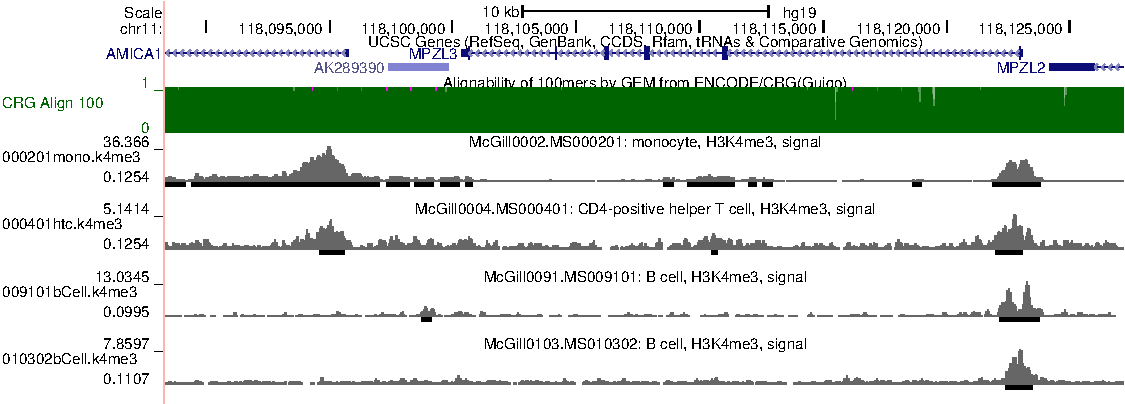
\includegraphics[width=\textwidth]{screenshot-ucsc-edited}

  \begin{itemize}
  \item Grey profiles are noisy aligned read count signals -- \\peaks
    are genomic locations with protein binding sites.
  \item Black bars are peaks called by MACS2 (Zhang et al, 2008) -- many
    false positives! (black bars where there is only noise)
  \item From a machine learning perspective, this could be binary
    classification (positive=peaks, negative=noise).
  \item We treat this as a changepoint detection problem with two
    states.
  \end{itemize}
\end{frame}

\begin{frame}
  \frametitle{Citation and new idea}
  Hocking TD, Rigaill G, Fearnhead P, Bourque G. Constrained Dynamic
  Programming and Supervised Penalty Learning Algorithms for Peak
  Detection in Genomic Data. Journal of Machine Learning Research
  21(87):1-40, 2020.

  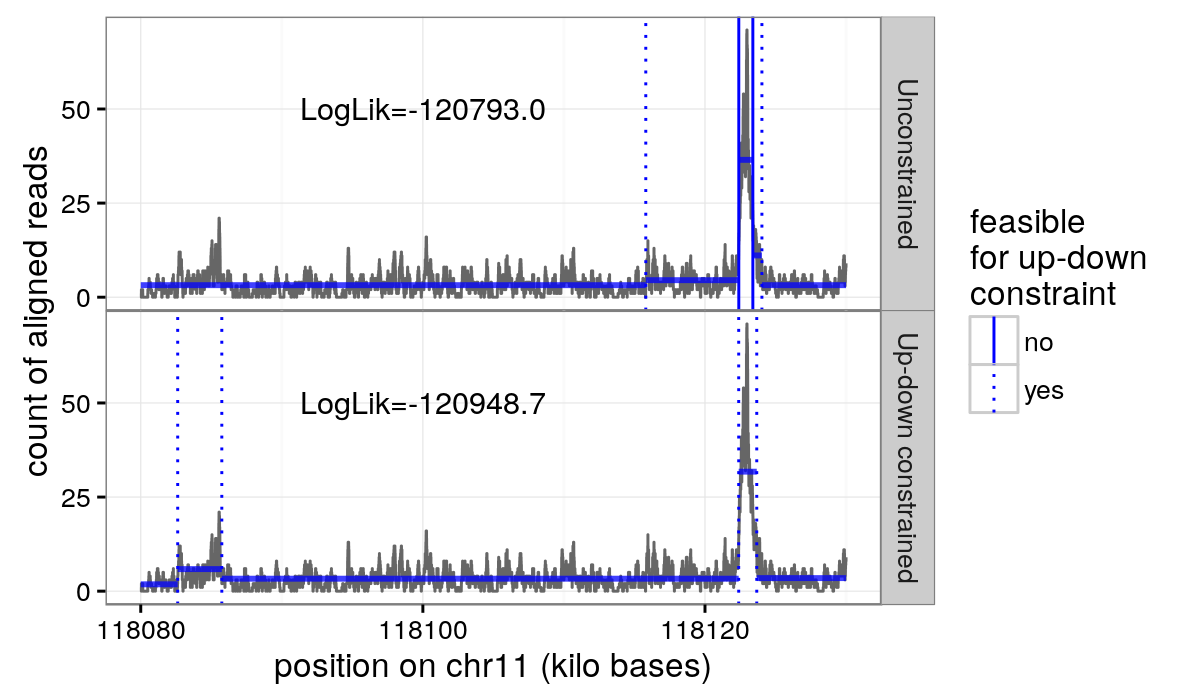
\includegraphics[width=0.8\textwidth]{figure-data-models}

  New idea: an optimal algorithm for computing best
  changepoints which alternate up and down (R package PeakSegOptimal).

\end{frame}

\begin{frame}
  \frametitle{Comparison to previous work and novelty}
{  \scriptsize
    \begin{tabular}{r|c|c}
    Constraint & No pruning & Functional pruning \\
    \hline
    None & Dynamic Prog. Algo. (DPA) & Pruned DPA (PDPA) \\
    & Optimal, $O(Sn^2)$ time & Optimal, $O(Sn\log n)$ time\\
    & Auger and Lawrence (1989) & Rigaill (2010); Johnson (2011) \\
    \hline
    Up-down & Constrained DPA (CDPA) & Generalized Pruned DPA (GPDPA) \\
    & Sub-optimal, $O(Sn^2)$ time & Optimal, $O(Sn\log n)$ time\\
    & Hocking et al. (2015) & \textbf{This paper} \\
    \hline
  \end{tabular}
}
\vspace{-0.3cm}
\begin{align*}
    \minimize_{\substack{
  \mathbf u\in\RR^{S}
\\
   0=t_0<t_1<\cdots<t_{S-1}<t_S=n
  }} &\ \ 
    \sum_{s=1}^S\  \sum_{i=1+t_{s-1}}^{t_s} \ell( u_s,  z_i) 
\\
      \text{subject to \hskip 0.75cm} &\ \ \alert{u_{s-1} \leq u_s\ \forall s\in\{2,4,\dots\},}
  \nonumber\\
  &\ \ \alert{u_{s-1} \geq u_s\ \forall s\in\{3,5,\dots\}.}
  \nonumber 
\end{align*}
\vskip -0.4cm
\begin{itemize}  
\item Let there be a sequence of $n$ data: $z_1,\dots,z_n$, and corresponding loss function $\ell$ (for example, Poisson loss for non-negative count data).
\item One hyper-parameter = number of segments $S\in\{1,3,\dots\}$.
\item \alert{Up-down constraints: $P=(S-1)/2$ peaks.}
\item Discrete/non-convex problem, naively $O(n^S)$ time.
\item Main novelty: fast and optimal algorithm for this
  problem.
\end{itemize}


\end{frame}

\begin{frame}
  \frametitle{Labeled data setting, learning to predict penalty}

  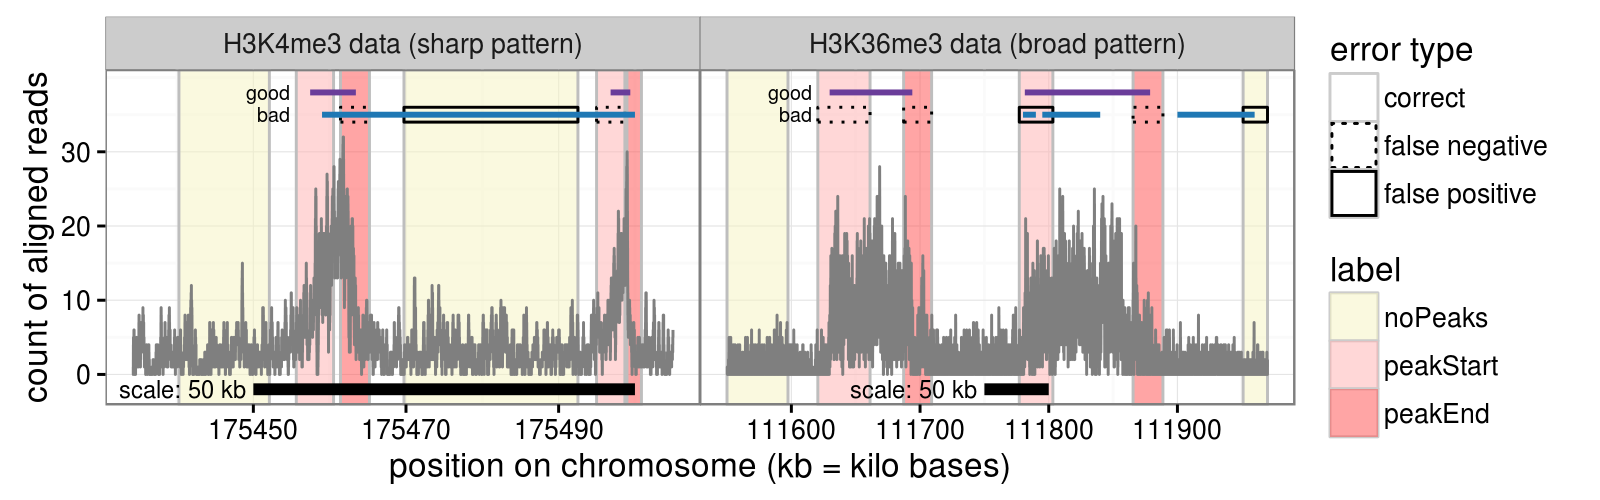
\includegraphics[width=\textwidth]{figure-good-bad}

  \begin{itemize}
  \item 2752 expert-labeled sequences (H {\it et al.}, {\it Bioinformatics} 2017). 
    {\small \url{https://rcdata.nau.edu/genomic-ml/chip-seq-chunk-db/}}
  \item Split sequences into train and test, learn using labels in
    train set, then predict peaks on test set.
    \begin{itemize}
    \item  If we have optimal loss $L_s$ for model size $s$,
    \item then for penalty $\lambda\geq 0$ we select the model of size $ S^*(\lambda) = \argmin_s L_s + \lambda s $ (standard linear penalty in statistics).
    \item We compute a fixed feature vector $x$ for each sequence,
      then learn $f(x)=\log \lambda$ to minimize a convex relaxation of label
      error. (H. \emph{et al.}, ICML'13)
    \end{itemize}
\end{itemize}

\end{frame}

\begin{frame}
  \frametitle{Test ROC curves of predicted peaks}
  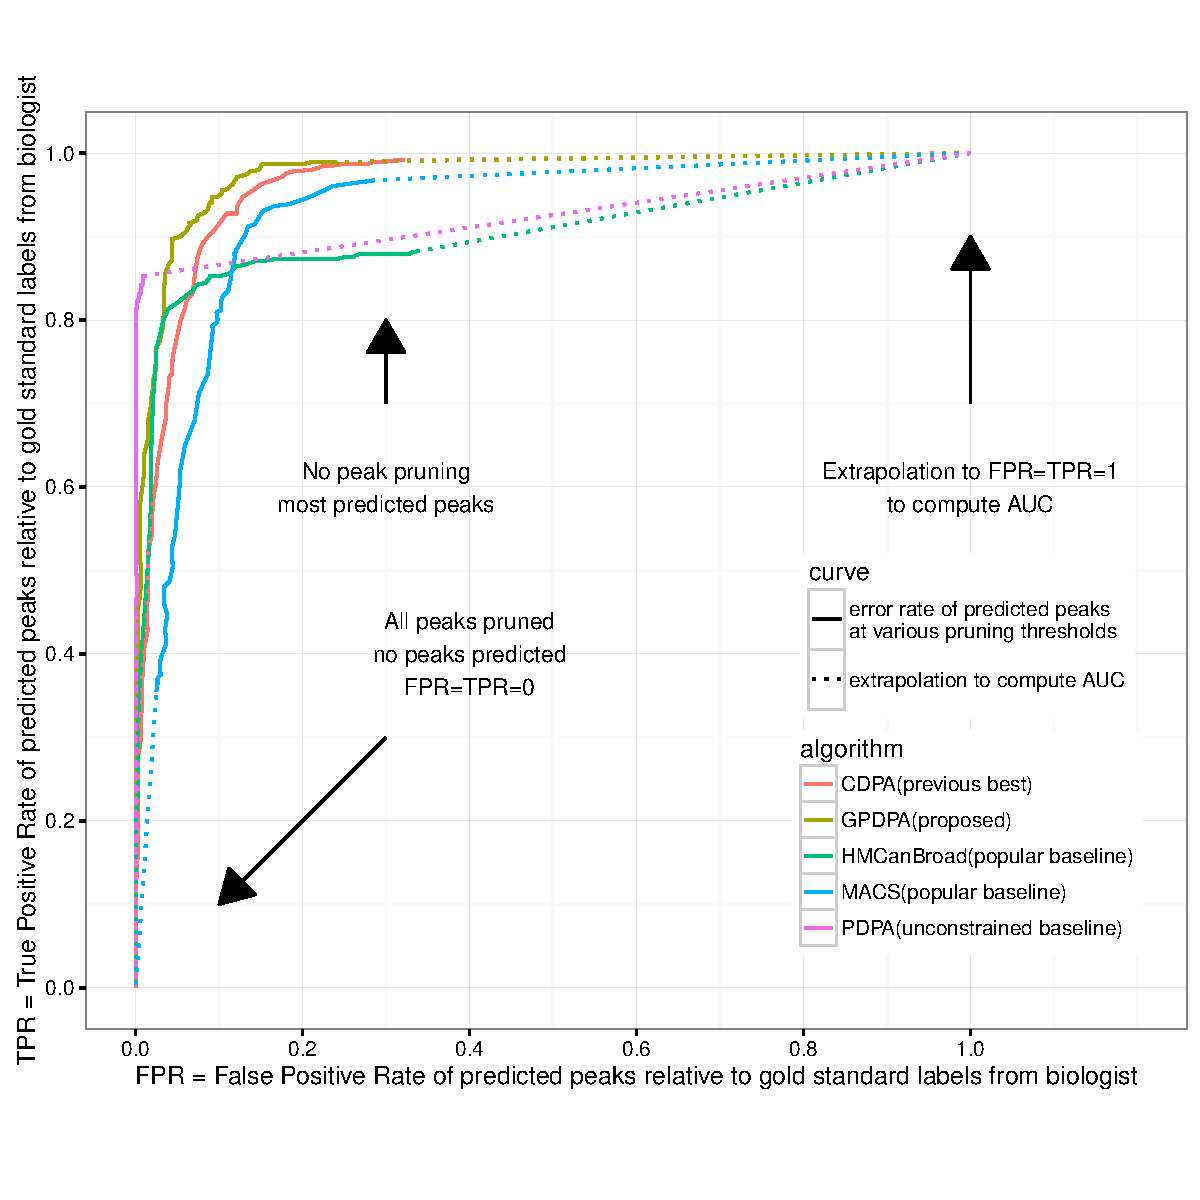
\includegraphics[width=0.8\textwidth]{figure-test-error-dots-ROC-supp.pdf}

  Each point on the ROC curve corresponds to a different penalty $\lambda$.
\end{frame}

\begin{frame}
  \frametitle{Test AUC of predicted peaks}
  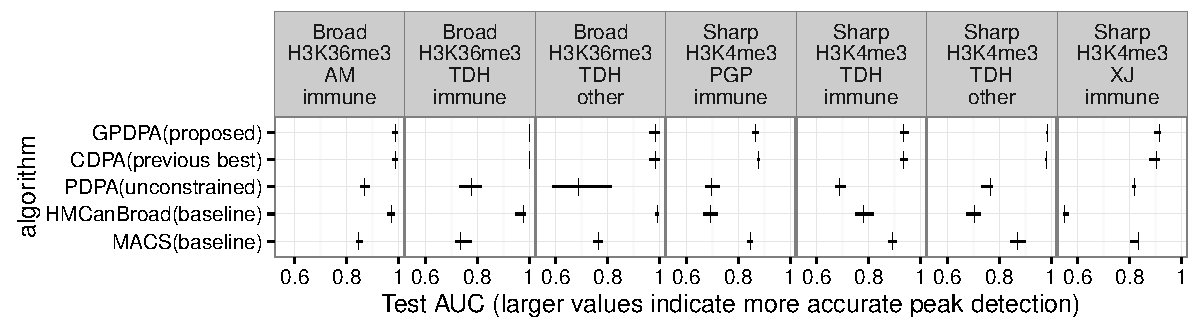
\includegraphics[width=\textwidth]{figure-test-error-dots}
  \begin{itemize}
  \item 4-fold cross-validation: train on 3/4 of labels, test on 1/4.
  \item All models trained by learning a scalar significance
    threshold / penalty parameter, which is varied to compute ROC/AUC.
  \item MACS is highly inaccurate in all data sets.
  \item HMCanBroad is accurate for broad but not sharp pattern.
  \item Unconstrained PDPA algorithm not as accurate as up-down
    constrained algorithms (CDPA, GPDPA).
  \end{itemize}
  \scriptsize
  %\url{http://bl.ocks.org/tdhock/raw/886575874144c3b172ce6b7d7d770b9f/} 
\end{frame}


\begin{frame}
  \frametitle{Time complexity analysis 1 (real genomic ChIP-seq data)}
  
  % Created by tikzDevice version 0.12 on 2018-12-06 14:46:08
% !TEX encoding = UTF-8 Unicode
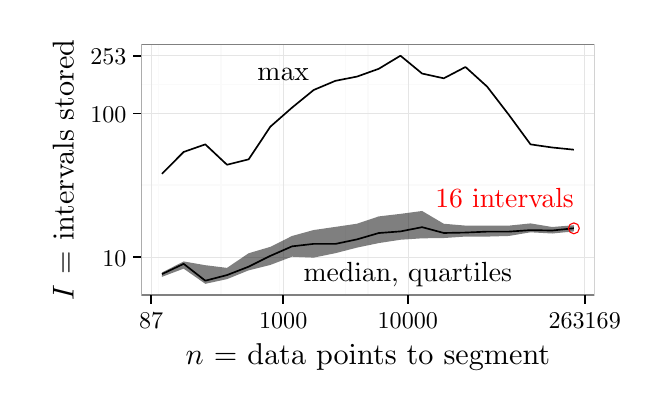
\begin{tikzpicture}[x=1pt,y=1pt]
\definecolor{fillColor}{RGB}{255,255,255}
\path[use as bounding box,fill=fillColor,fill opacity=0.00] (0,0) rectangle (216.81,130.09);
\begin{scope}
\path[clip] (  0.00,  0.00) rectangle (216.81,130.09);
\definecolor{drawColor}{RGB}{255,255,255}
\definecolor{fillColor}{RGB}{255,255,255}

\path[draw=drawColor,line width= 0.6pt,line join=round,line cap=round,fill=fillColor] ( -0.00,  0.00) rectangle (216.81,130.09);
\end{scope}
\begin{scope}
\path[clip] ( 41.08, 33.41) rectangle (204.81,124.09);
\definecolor{fillColor}{RGB}{255,255,255}

\path[fill=fillColor] ( 41.08, 33.41) rectangle (204.81,124.09);
\definecolor{drawColor}{gray}{0.98}

\path[draw=drawColor,line width= 0.6pt,line join=round] ( 41.08, 73.12) --
	(204.81, 73.12);

\path[draw=drawColor,line width= 0.6pt,line join=round] ( 41.08,109.51) --
	(204.81,109.51);

\path[draw=drawColor,line width= 0.6pt,line join=round] ( 47.33, 33.41) --
	( 47.33,124.09);

\path[draw=drawColor,line width= 0.6pt,line join=round] ( 69.83, 33.41) --
	( 69.83,124.09);

\path[draw=drawColor,line width= 0.6pt,line join=round] (114.85, 33.41) --
	(114.85,124.09);

\path[draw=drawColor,line width= 0.6pt,line join=round] ( 90.98, 33.41) --
	( 90.98,124.09);

\path[draw=drawColor,line width= 0.6pt,line join=round] (122.95, 33.41) --
	(122.95,124.09);
\definecolor{drawColor}{gray}{0.90}

\path[draw=drawColor,line width= 0.2pt,line join=round] ( 41.08, 47.19) --
	(204.81, 47.19);

\path[draw=drawColor,line width= 0.2pt,line join=round] ( 41.08, 99.06) --
	(204.81, 99.06);

\path[draw=drawColor,line width= 0.2pt,line join=round] ( 41.08,119.96) --
	(204.81,119.96);

\path[draw=drawColor,line width= 0.2pt,line join=round] ( 92.34, 33.41) --
	( 92.34,124.09);

\path[draw=drawColor,line width= 0.2pt,line join=round] (137.36, 33.41) --
	(137.36,124.09);

\path[draw=drawColor,line width= 0.2pt,line join=round] ( 44.61, 33.41) --
	( 44.61,124.09);

\path[draw=drawColor,line width= 0.2pt,line join=round] (201.28, 33.41) --
	(201.28,124.09);
\definecolor{drawColor}{RGB}{0,0,0}

\node[text=drawColor,anchor=base,inner sep=0pt, outer sep=0pt, scale=  1.00] at ( 92.34,110.83) {max};

\node[text=drawColor,anchor=base,inner sep=0pt, outer sep=0pt, scale=  1.00] at (137.36, 38.38) {median, quartiles};

\path[draw=drawColor,line width= 0.6pt,line join=round] ( 48.52, 77.26) --
	( 56.36, 85.18) --
	( 64.19, 87.92) --
	( 72.02, 80.56) --
	( 79.86, 82.52) --
	( 87.69, 94.31) --
	( 95.53,101.20) --
	(103.36,107.58) --
	(111.19,110.88) --
	(119.03,112.42) --
	(126.86,115.23) --
	(134.70,119.96) --
	(142.53,113.51) --
	(150.36,111.79) --
	(158.20,115.88) --
	(166.03,108.78) --
	(173.87, 98.60) --
	(181.70, 87.92) --
	(189.53, 86.79) --
	(197.37, 86.00);
\definecolor{fillColor}{RGB}{0,0,0}

\path[fill=fillColor,fill opacity=0.50] ( 48.52, 41.61) --
	( 56.36, 45.62) --
	( 64.19, 44.26) --
	( 72.02, 43.29) --
	( 79.86, 48.58) --
	( 87.69, 50.89) --
	( 95.53, 54.82) --
	(103.36, 56.97) --
	(111.19, 58.10) --
	(119.03, 59.25) --
	(126.86, 61.89) --
	(134.70, 62.81) --
	(142.53, 63.85) --
	(150.36, 59.23) --
	(158.20, 58.57) --
	(166.03, 58.52) --
	(173.87, 58.56) --
	(181.70, 59.36) --
	(189.53, 58.06) --
	(197.37, 58.70) --
	(197.37, 56.47) --
	(189.53, 55.71) --
	(181.70, 56.15) --
	(173.87, 54.82) --
	(166.03, 54.60) --
	(158.20, 54.61) --
	(150.36, 54.07) --
	(142.53, 53.97) --
	(134.70, 53.45) --
	(126.86, 52.25) --
	(119.03, 50.62) --
	(111.19, 48.60) --
	(103.36, 47.00) --
	( 95.53, 47.33) --
	( 87.69, 44.36) --
	( 79.86, 42.40) --
	( 72.02, 39.22) --
	( 64.19, 37.53) --
	( 56.36, 43.01) --
	( 48.52, 40.05) --
	cycle;

\path[draw=drawColor,line width= 0.6pt,line join=round] ( 48.52, 41.04) --
	( 56.36, 44.75) --
	( 64.19, 38.66) --
	( 72.02, 40.69) --
	( 79.86, 43.73) --
	( 87.69, 47.63) --
	( 95.53, 51.07) --
	(103.36, 51.97) --
	(111.19, 51.95) --
	(119.03, 53.60) --
	(126.86, 55.88) --
	(134.70, 56.47) --
	(142.53, 58.00) --
	(150.36, 55.90) --
	(158.20, 56.05) --
	(166.03, 56.39) --
	(173.87, 56.39) --
	(181.70, 56.94) --
	(189.53, 56.79) --
	(197.37, 57.61);
\definecolor{drawColor}{RGB}{255,0,0}

\path[draw=drawColor,line width= 0.4pt,line join=round,line cap=round] (197.37, 57.58) circle (  1.96);

\node[text=drawColor,anchor=base east,inner sep=0pt, outer sep=0pt, scale=  1.00] at (197.37, 65.15) {16 intervals};
\definecolor{drawColor}{gray}{0.50}

\path[draw=drawColor,line width= 0.6pt,line join=round,line cap=round] ( 41.08, 33.41) rectangle (204.81,124.09);
\end{scope}
\begin{scope}
\path[clip] (  0.00,  0.00) rectangle (216.81,130.09);
\definecolor{drawColor}{RGB}{0,0,0}

\node[text=drawColor,anchor=base east,inner sep=0pt, outer sep=0pt, scale=  0.87] at ( 35.68, 43.90) {10};

\node[text=drawColor,anchor=base east,inner sep=0pt, outer sep=0pt, scale=  0.87] at ( 35.68, 95.77) {100};

\node[text=drawColor,anchor=base east,inner sep=0pt, outer sep=0pt, scale=  0.87] at ( 35.68,116.67) {253};
\end{scope}
\begin{scope}
\path[clip] (  0.00,  0.00) rectangle (216.81,130.09);
\definecolor{drawColor}{RGB}{0,0,0}

\path[draw=drawColor,line width= 0.6pt,line join=round] ( 38.08, 47.19) --
	( 41.08, 47.19);

\path[draw=drawColor,line width= 0.6pt,line join=round] ( 38.08, 99.06) --
	( 41.08, 99.06);

\path[draw=drawColor,line width= 0.6pt,line join=round] ( 38.08,119.96) --
	( 41.08,119.96);
\end{scope}
\begin{scope}
\path[clip] (  0.00,  0.00) rectangle (216.81,130.09);
\definecolor{drawColor}{RGB}{0,0,0}

\path[draw=drawColor,line width= 0.6pt,line join=round] ( 92.34, 30.41) --
	( 92.34, 33.41);

\path[draw=drawColor,line width= 0.6pt,line join=round] (137.36, 30.41) --
	(137.36, 33.41);

\path[draw=drawColor,line width= 0.6pt,line join=round] ( 44.61, 30.41) --
	( 44.61, 33.41);

\path[draw=drawColor,line width= 0.6pt,line join=round] (201.28, 30.41) --
	(201.28, 33.41);
\end{scope}
\begin{scope}
\path[clip] (  0.00,  0.00) rectangle (216.81,130.09);
\definecolor{drawColor}{RGB}{0,0,0}

\node[text=drawColor,anchor=base,inner sep=0pt, outer sep=0pt, scale=  0.87] at ( 92.34, 21.43) {1000};

\node[text=drawColor,anchor=base,inner sep=0pt, outer sep=0pt, scale=  0.87] at (137.36, 21.43) {10000};

\node[text=drawColor,anchor=base,inner sep=0pt, outer sep=0pt, scale=  0.87] at ( 44.61, 21.43) {87};

\node[text=drawColor,anchor=base,inner sep=0pt, outer sep=0pt, scale=  0.87] at (201.28, 21.43) {263169};
\end{scope}
\begin{scope}
\path[clip] (  0.00,  0.00) rectangle (216.81,130.09);
\definecolor{drawColor}{RGB}{0,0,0}

\node[text=drawColor,anchor=base,inner sep=0pt, outer sep=0pt, scale=  1.09] at (122.95,  8.40) {$n$ = data points to segment};
\end{scope}
\begin{scope}
\path[clip] (  0.00,  0.00) rectangle (216.81,130.09);
\definecolor{drawColor}{RGB}{0,0,0}

\node[text=drawColor,rotate= 90.00,anchor=base,inner sep=0pt, outer sep=0pt, scale=  1.09] at ( 16.63, 78.75) {$I$ = intervals stored};
\end{scope}
\end{tikzpicture}


  \begin{itemize}
  \item Dynamic programming algorithm uses functional pruning, which
    requires storing the cost as a function of the last segment mean.
  \item This cost function can be computed/stored exactly in terms of
    several pieces/intervals with different coefficients.
  \item The algorithm complexity is linear in the number of intervals,
    and the figure above shows that it is very small, $O(\log n)$, for
    real data, much smaller than worst case $O(n)$.
  \end{itemize}

\end{frame}

\begin{frame}
  \frametitle{Time complexity analysis 2 (real genomic ChIP-seq data)}
  
  % Created by tikzDevice version 0.10.1 on 2017-06-14 16:11:18
% !TEX encoding = UTF-8 Unicode
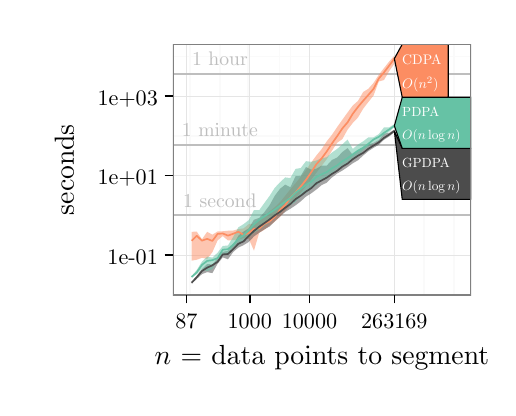
\begin{tikzpicture}[x=1pt,y=1pt]
\definecolor{fillColor}{RGB}{255,255,255}
\path[use as bounding box,fill=fillColor,fill opacity=0.00] (0,0) rectangle (166.22,130.09);
\begin{scope}
\path[clip] (  0.00,  0.00) rectangle (166.22,130.09);
\definecolor{drawColor}{RGB}{255,255,255}
\definecolor{fillColor}{RGB}{255,255,255}

\path[draw=drawColor,line width= 0.6pt,line join=round,line cap=round,fill=fillColor] (  0.00,  0.00) rectangle (166.22,130.09);
\end{scope}
\begin{scope}
\path[clip] ( 52.45, 33.48) rectangle (160.22,124.09);
\definecolor{fillColor}{RGB}{255,255,255}

\path[fill=fillColor] ( 52.45, 33.48) rectangle (160.22,124.09);
\definecolor{drawColor}{gray}{0.98}

\path[draw=drawColor,line width= 0.6pt,line join=round] ( 52.45, 33.60) --
	(160.22, 33.60);

\path[draw=drawColor,line width= 0.6pt,line join=round] ( 52.45, 62.29) --
	(160.22, 62.29);

\path[draw=drawColor,line width= 0.6pt,line join=round] ( 52.45, 90.99) --
	(160.22, 90.99);

\path[draw=drawColor,line width= 0.6pt,line join=round] ( 52.45,119.68) --
	(160.22,119.68);

\path[draw=drawColor,line width= 0.6pt,line join=round] ( 58.65, 33.48) --
	( 58.65,124.09);

\path[draw=drawColor,line width= 0.6pt,line join=round] ( 69.45, 33.48) --
	( 69.45,124.09);

\path[draw=drawColor,line width= 0.6pt,line join=round] ( 91.04, 33.48) --
	( 91.04,124.09);

\path[draw=drawColor,line width= 0.6pt,line join=round] ( 79.59, 33.48) --
	( 79.59,124.09);

\path[draw=drawColor,line width= 0.6pt,line join=round] ( 94.92, 33.48) --
	( 94.92,124.09);

\path[draw=drawColor,line width= 0.6pt,line join=round] (143.30, 33.48) --
	(143.30,124.09);

\path[draw=drawColor,line width= 0.6pt,line join=round] (154.09, 33.48) --
	(154.09,124.09);
\definecolor{drawColor}{gray}{0.90}

\path[draw=drawColor,line width= 0.2pt,line join=round] ( 52.45, 47.94) --
	(160.22, 47.94);

\path[draw=drawColor,line width= 0.2pt,line join=round] ( 52.45, 76.64) --
	(160.22, 76.64);

\path[draw=drawColor,line width= 0.2pt,line join=round] ( 52.45,105.34) --
	(160.22,105.34);

\path[draw=drawColor,line width= 0.2pt,line join=round] ( 80.24, 33.48) --
	( 80.24,124.09);

\path[draw=drawColor,line width= 0.2pt,line join=round] (101.84, 33.48) --
	(101.84,124.09);

\path[draw=drawColor,line width= 0.2pt,line join=round] ( 57.35, 33.48) --
	( 57.35,124.09);

\path[draw=drawColor,line width= 0.2pt,line join=round] (132.50, 33.48) --
	(132.50,124.09);
\definecolor{drawColor}{RGB}{190,190,190}

\path[draw=drawColor,line width= 0.6pt,line join=round] ( 52.45, 62.29) -- (160.22, 62.29);

\path[draw=drawColor,line width= 0.6pt,line join=round] ( 52.45, 87.80) -- (160.22, 87.80);

\path[draw=drawColor,line width= 0.6pt,line join=round] ( 52.45,113.32) -- (160.22,113.32);
\definecolor{fillColor}{RGB}{252,141,98}

\path[fill=fillColor,fill opacity=0.50] ( 59.23, 56.31) --
	( 61.10, 56.41) --
	( 62.98, 53.63) --
	( 64.86, 56.33) --
	( 66.74, 55.29) --
	( 68.62, 56.44) --
	( 70.50, 56.53) --
	( 72.38, 56.71) --
	( 74.26, 56.77) --
	( 76.14, 57.32) --
	( 78.01, 57.55) --
	( 79.89, 59.09) --
	( 81.77, 59.27) --
	( 83.65, 60.25) --
	( 85.53, 61.93) --
	( 87.41, 63.71) --
	( 89.29, 65.22) --
	( 91.17, 67.03) --
	( 93.05, 69.35) --
	( 94.92, 71.70) --
	( 96.80, 73.89) --
	( 98.68, 76.20) --
	(100.56, 78.62) --
	(102.44, 81.34) --
	(104.32, 83.90) --
	(106.20, 86.17) --
	(108.08, 89.06) --
	(109.96, 91.40) --
	(111.83, 94.17) --
	(113.71, 96.82) --
	(115.59, 99.43) --
	(117.47,101.96) --
	(119.35,103.61) --
	(121.23,106.85) --
	(123.11,108.01) --
	(124.99,110.14) --
	(126.87,113.05) --
	(128.74,115.46) --
	(130.62,117.84) --
	(132.50,119.97) --
	(132.50,117.05) --
	(130.62,114.38) --
	(128.74,111.17) --
	(126.87,110.63) --
	(124.99,105.59) --
	(123.11,103.24) --
	(121.23,100.79) --
	(119.35, 97.63) --
	(117.47, 95.66) --
	(115.59, 93.22) --
	(113.71, 89.83) --
	(111.83, 88.50) --
	(109.96, 85.63) --
	(108.08, 82.61) --
	(106.20, 80.12) --
	(104.32, 77.65) --
	(102.44, 75.15) --
	(100.56, 72.82) --
	( 98.68, 70.51) --
	( 96.80, 68.28) --
	( 94.92, 65.92) --
	( 93.05, 63.83) --
	( 91.17, 61.72) --
	( 89.29, 60.00) --
	( 87.41, 58.57) --
	( 85.53, 57.08) --
	( 83.65, 55.93) --
	( 81.77, 49.53) --
	( 79.89, 53.78) --
	( 78.01, 54.02) --
	( 76.14, 53.50) --
	( 74.26, 53.32) --
	( 72.38, 53.21) --
	( 70.50, 54.79) --
	( 68.62, 53.21) --
	( 66.74, 48.97) --
	( 64.86, 46.55) --
	( 62.98, 46.93) --
	( 61.10, 46.23) --
	( 59.23, 45.90) --
	cycle;
\definecolor{fillColor}{RGB}{77,77,77}

\path[fill=fillColor,fill opacity=0.50] ( 59.23, 38.22) --
	( 61.10, 40.44) --
	( 62.98, 42.83) --
	( 64.86, 44.66) --
	( 66.74, 44.55) --
	( 68.62, 46.78) --
	( 70.50, 49.08) --
	( 72.38, 49.48) --
	( 74.26, 51.50) --
	( 76.14, 54.93) --
	( 78.01, 56.41) --
	( 79.89, 57.59) --
	( 81.77, 60.70) --
	( 83.65, 61.34) --
	( 85.53, 63.44) --
	( 87.41, 65.92) --
	( 89.29, 69.35) --
	( 91.17, 71.84) --
	( 93.05, 73.37) --
	( 94.92, 72.43) --
	( 96.80, 76.42) --
	( 98.68, 76.52) --
	(100.56, 79.73) --
	(102.44, 78.79) --
	(104.32, 79.14) --
	(106.20, 80.25) --
	(108.08, 80.26) --
	(109.96, 82.28) --
	(111.83, 83.17) --
	(113.71, 85.16) --
	(115.59, 86.58) --
	(117.47, 84.11) --
	(119.35, 85.53) --
	(121.23, 86.82) --
	(123.11, 87.95) --
	(124.99, 88.45) --
	(126.87, 89.50) --
	(128.74, 91.81) --
	(130.62, 92.09) --
	(132.50, 93.26) --
	(132.50, 92.31) --
	(130.62, 90.78) --
	(128.74, 89.57) --
	(126.87, 87.77) --
	(124.99, 86.69) --
	(123.11, 85.47) --
	(121.23, 83.89) --
	(119.35, 82.17) --
	(117.47, 81.08) --
	(115.59, 79.71) --
	(113.71, 78.46) --
	(111.83, 77.38) --
	(109.96, 75.95) --
	(108.08, 74.09) --
	(106.20, 73.18) --
	(104.32, 71.62) --
	(102.44, 70.21) --
	(100.56, 69.05) --
	( 98.68, 67.34) --
	( 96.80, 65.88) --
	( 94.92, 64.65) --
	( 93.05, 63.48) --
	( 91.17, 61.86) --
	( 89.29, 60.13) --
	( 87.41, 58.25) --
	( 85.53, 57.19) --
	( 83.65, 55.98) --
	( 81.77, 54.64) --
	( 79.89, 52.66) --
	( 78.01, 51.50) --
	( 76.14, 50.63) --
	( 74.26, 49.03) --
	( 72.38, 46.40) --
	( 70.50, 47.08) --
	( 68.62, 44.76) --
	( 66.74, 41.40) --
	( 64.86, 41.75) --
	( 62.98, 41.04) --
	( 61.10, 39.31) --
	( 59.23, 37.60) --
	cycle;
\definecolor{fillColor}{RGB}{102,194,165}

\path[fill=fillColor,fill opacity=0.50] ( 59.23, 40.23) --
	( 61.10, 42.54) --
	( 62.98, 45.54) --
	( 64.86, 47.36) --
	( 66.74, 47.00) --
	( 68.62, 48.76) --
	( 70.50, 51.21) --
	( 72.38, 51.39) --
	( 74.26, 54.47) --
	( 76.14, 57.95) --
	( 78.01, 59.09) --
	( 79.89, 60.55) --
	( 81.77, 64.19) --
	( 83.65, 64.13) --
	( 85.53, 66.73) --
	( 87.41, 69.29) --
	( 89.29, 72.23) --
	( 91.17, 74.19) --
	( 93.05, 75.98) --
	( 94.92, 75.75) --
	( 96.80, 79.06) --
	( 98.68, 79.38) --
	(100.56, 81.85) --
	(102.44, 81.61) --
	(104.32, 82.09) --
	(106.20, 82.89) --
	(108.08, 83.27) --
	(109.96, 84.96) --
	(111.83, 86.27) --
	(113.71, 87.91) --
	(115.59, 89.65) --
	(117.47, 86.27) --
	(119.35, 87.83) --
	(121.23, 89.02) --
	(123.11, 90.45) --
	(124.99, 90.47) --
	(126.87, 91.61) --
	(128.74, 94.03) --
	(130.62, 94.05) --
	(132.50, 95.26) --
	(132.50, 94.21) --
	(130.62, 92.46) --
	(128.74, 91.15) --
	(126.87, 89.18) --
	(124.99, 88.33) --
	(123.11, 87.05) --
	(121.23, 85.70) --
	(119.35, 83.73) --
	(117.47, 82.47) --
	(115.59, 81.40) --
	(113.71, 80.04) --
	(111.83, 79.04) --
	(109.96, 77.51) --
	(108.08, 75.46) --
	(106.20, 74.73) --
	(104.32, 73.12) --
	(102.44, 71.77) --
	(100.56, 70.33) --
	( 98.68, 69.10) --
	( 96.80, 67.11) --
	( 94.92, 65.96) --
	( 93.05, 64.97) --
	( 91.17, 63.04) --
	( 89.29, 61.79) --
	( 87.41, 59.65) --
	( 85.53, 58.43) --
	( 83.65, 57.03) --
	( 81.77, 55.96) --
	( 79.89, 54.27) --
	( 78.01, 53.42) --
	( 76.14, 51.39) --
	( 74.26, 50.63) --
	( 72.38, 48.07) --
	( 70.50, 48.13) --
	( 68.62, 46.40) --
	( 66.74, 42.83) --
	( 64.86, 42.08) --
	( 62.98, 42.83) --
	( 61.10, 41.04) --
	( 59.23, 39.78) --
	cycle;
\definecolor{drawColor}{RGB}{252,141,98}

\path[draw=drawColor,line width= 0.6pt,line join=round] ( 59.23, 53.07) --
	( 61.10, 54.88) --
	( 62.98, 53.13) --
	( 64.86, 53.78) --
	( 66.74, 53.02) --
	( 68.62, 55.57) --
	( 70.50, 55.72) --
	( 72.38, 54.95) --
	( 74.26, 55.62) --
	( 76.14, 56.36) --
	( 78.01, 55.24) --
	( 79.89, 55.87) --
	( 81.77, 57.41) --
	( 83.65, 57.49) --
	( 85.53, 59.16) --
	( 87.41, 60.08) --
	( 89.29, 61.78) --
	( 91.17, 64.16) --
	( 93.05, 66.01) --
	( 94.92, 68.66) --
	( 96.80, 70.54) --
	( 98.68, 72.71) --
	(100.56, 75.08) --
	(102.44, 77.81) --
	(104.32, 80.75) --
	(106.20, 82.83) --
	(108.08, 85.37) --
	(109.96, 88.25) --
	(111.83, 90.88) --
	(113.71, 93.69) --
	(115.59, 95.87) --
	(117.47, 98.97) --
	(119.35,101.44) --
	(121.23,103.68) --
	(123.11,105.79) --
	(124.99,108.00) --
	(126.87,111.70) --
	(128.74,113.91) --
	(130.62,116.37) --
	(132.50,118.90);
\definecolor{drawColor}{gray}{0.30}

\path[draw=drawColor,line width= 0.6pt,line join=round] ( 59.23, 37.91) --
	( 61.10, 39.90) --
	( 62.98, 42.16) --
	( 64.86, 43.37) --
	( 66.74, 44.22) --
	( 68.62, 45.49) --
	( 70.50, 48.16) --
	( 72.38, 48.31) --
	( 74.26, 50.08) --
	( 76.14, 52.01) --
	( 78.01, 52.88) --
	( 79.89, 54.84) --
	( 81.77, 56.64) --
	( 83.65, 58.16) --
	( 85.53, 59.46) --
	( 87.41, 60.80) --
	( 89.29, 62.26) --
	( 91.17, 63.52) --
	( 93.05, 65.03) --
	( 94.92, 66.36) --
	( 96.80, 68.12) --
	( 98.68, 69.37) --
	(100.56, 70.86) --
	(102.44, 72.08) --
	(104.32, 73.87) --
	(106.20, 74.89) --
	(108.08, 75.91) --
	(109.96, 77.25) --
	(111.83, 78.37) --
	(113.71, 79.89) --
	(115.59, 80.98) --
	(117.47, 82.57) --
	(119.35, 83.82) --
	(121.23, 84.85) --
	(123.11, 86.34) --
	(124.99, 87.50) --
	(126.87, 88.67) --
	(128.74, 90.26) --
	(130.62, 91.44) --
	(132.50, 92.78);
\definecolor{drawColor}{RGB}{102,194,165}

\path[draw=drawColor,line width= 0.6pt,line join=round] ( 59.23, 40.01) --
	( 61.10, 41.66) --
	( 62.98, 44.39) --
	( 64.86, 45.81) --
	( 66.74, 46.07) --
	( 68.62, 46.82) --
	( 70.50, 49.86) --
	( 72.38, 50.04) --
	( 74.26, 51.67) --
	( 76.14, 53.83) --
	( 78.01, 55.06) --
	( 79.89, 56.95) --
	( 81.77, 59.02) --
	( 83.65, 60.66) --
	( 85.53, 61.85) --
	( 87.41, 63.17) --
	( 89.29, 64.32) --
	( 91.17, 65.76) --
	( 93.05, 67.22) --
	( 94.92, 68.54) --
	( 96.80, 70.45) --
	( 98.68, 71.88) --
	(100.56, 73.31) --
	(102.44, 74.39) --
	(104.32, 76.12) --
	(106.20, 77.09) --
	(108.08, 77.91) --
	(109.96, 79.28) --
	(111.83, 80.29) --
	(113.71, 81.85) --
	(115.59, 82.92) --
	(117.47, 84.31) --
	(119.35, 85.66) --
	(121.23, 86.72) --
	(123.11, 88.11) --
	(124.99, 89.70) --
	(126.87, 90.62) --
	(128.74, 92.08) --
	(130.62, 93.31) --
	(132.50, 94.60);
\definecolor{drawColor}{RGB}{190,190,190}

\node[text=drawColor,anchor=base,inner sep=0pt, outer sep=0pt, scale=  0.71] at ( 69.45, 65.23) {1 second};

\node[text=drawColor,anchor=base,inner sep=0pt, outer sep=0pt, scale=  0.71] at ( 69.45, 90.74) {1 minute};

\node[text=drawColor,anchor=base,inner sep=0pt, outer sep=0pt, scale=  0.71] at ( 69.45,116.26) {1 hour};
\end{scope}
\begin{scope}
\path[clip] ( 52.45, 33.48) rectangle (160.22,124.09);
\definecolor{drawColor}{RGB}{0,0,0}
\definecolor{fillColor}{gray}{0.30}

\path[draw=drawColor,line width= 0.4pt,line join=round,line cap=round,fill=fillColor] (132.50, 92.78) --
	(135.35, 86.47) --
	(160.22, 86.47) --
	(160.22, 68.02) --
	(135.35, 68.02) --
	cycle;
\definecolor{fillColor}{RGB}{102,194,165}

\path[draw=drawColor,line width= 0.4pt,line join=round,line cap=round,fill=fillColor] (132.50, 94.60) --
	(135.35,104.93) --
	(160.22,104.93) --
	(160.22, 86.47) --
	(135.35, 86.47) --
	cycle;
\definecolor{fillColor}{RGB}{252,141,98}

\path[draw=drawColor,line width= 0.4pt,line join=round,line cap=round,fill=fillColor] (132.50,118.90) --
	(135.35,124.09) --
	(151.98,124.09) --
	(151.98,104.93) --
	(135.35,104.93) --
	cycle;
\definecolor{drawColor}{RGB}{255,255,255}

\node[text=drawColor,anchor=base west,inner sep=0pt, outer sep=0pt, scale=  0.48] at (135.35, 79.42) {GPDPA};

\node[text=drawColor,anchor=base west,inner sep=0pt, outer sep=0pt, scale=  0.48] at (135.35, 71.10) {$O(n \log n)$};

\node[text=drawColor,anchor=base west,inner sep=0pt, outer sep=0pt, scale=  0.48] at (135.35, 97.87) {PDPA};

\node[text=drawColor,anchor=base west,inner sep=0pt, outer sep=0pt, scale=  0.48] at (135.35, 89.55) {$O(n \log n)$};

\node[text=drawColor,anchor=base west,inner sep=0pt, outer sep=0pt, scale=  0.50] at (135.35,116.76) {CDPA};

\node[text=drawColor,anchor=base west,inner sep=0pt, outer sep=0pt, scale=  0.50] at (135.35,108.12) {$O(n^2)$};
\definecolor{drawColor}{gray}{0.50}

\path[draw=drawColor,line width= 0.6pt,line join=round,line cap=round] ( 52.45, 33.48) rectangle (160.22,124.09);
\end{scope}
\begin{scope}
\path[clip] (  0.00,  0.00) rectangle (166.22,130.09);
\definecolor{drawColor}{RGB}{0,0,0}

\node[text=drawColor,anchor=base east,inner sep=0pt, outer sep=0pt, scale=  0.80] at ( 47.05, 44.64) {1e-01};

\node[text=drawColor,anchor=base east,inner sep=0pt, outer sep=0pt, scale=  0.80] at ( 47.05, 73.33) {1e+01};

\node[text=drawColor,anchor=base east,inner sep=0pt, outer sep=0pt, scale=  0.80] at ( 47.05,102.03) {1e+03};
\end{scope}
\begin{scope}
\path[clip] (  0.00,  0.00) rectangle (166.22,130.09);
\definecolor{drawColor}{RGB}{0,0,0}

\path[draw=drawColor,line width= 0.6pt,line join=round] ( 49.45, 47.94) --
	( 52.45, 47.94);

\path[draw=drawColor,line width= 0.6pt,line join=round] ( 49.45, 76.64) --
	( 52.45, 76.64);

\path[draw=drawColor,line width= 0.6pt,line join=round] ( 49.45,105.34) --
	( 52.45,105.34);
\end{scope}
\begin{scope}
\path[clip] (  0.00,  0.00) rectangle (166.22,130.09);
\definecolor{drawColor}{RGB}{0,0,0}

\path[draw=drawColor,line width= 0.6pt,line join=round] ( 80.24, 30.48) --
	( 80.24, 33.48);

\path[draw=drawColor,line width= 0.6pt,line join=round] (101.84, 30.48) --
	(101.84, 33.48);

\path[draw=drawColor,line width= 0.6pt,line join=round] ( 57.35, 30.48) --
	( 57.35, 33.48);

\path[draw=drawColor,line width= 0.6pt,line join=round] (132.50, 30.48) --
	(132.50, 33.48);
\end{scope}
\begin{scope}
\path[clip] (  0.00,  0.00) rectangle (166.22,130.09);
\definecolor{drawColor}{RGB}{0,0,0}

\node[text=drawColor,anchor=base,inner sep=0pt, outer sep=0pt, scale=  0.80] at ( 80.24, 21.46) {1000};

\node[text=drawColor,anchor=base,inner sep=0pt, outer sep=0pt, scale=  0.80] at (101.84, 21.46) {10000};

\node[text=drawColor,anchor=base,inner sep=0pt, outer sep=0pt, scale=  0.80] at ( 57.35, 21.46) {87};

\node[text=drawColor,anchor=base,inner sep=0pt, outer sep=0pt, scale=  0.80] at (132.50, 21.46) {263169};
\end{scope}
\begin{scope}
\path[clip] (  0.00,  0.00) rectangle (166.22,130.09);
\definecolor{drawColor}{RGB}{0,0,0}

\node[text=drawColor,anchor=base,inner sep=0pt, outer sep=0pt, scale=  1.00] at (106.33,  8.40) {$n$ = data points to segment};
\end{scope}
\begin{scope}
\path[clip] (  0.00,  0.00) rectangle (166.22,130.09);
\definecolor{drawColor}{RGB}{0,0,0}

\node[text=drawColor,rotate= 90.00,anchor=base,inner sep=0pt, outer sep=0pt, scale=  1.00] at ( 16.66, 78.78) {seconds};
\end{scope}
\end{tikzpicture}


  \begin{itemize}
  \item Computation time for a fixed number of peaks, 20.
  \item Proposed GPDPA with up-down constraints is just as fast as
    previous PDPA with no constraints between adjacent segment means.
  \item Both are much faster than the CDPA (heuristic/approximate
    algorithm which enforces up-down constraints).
  \end{itemize}

\end{frame}

\section{Generalized Functional Pruning Optimal Partitioning (GFPOP)
  for Constrained Changepoint Detection in Genomic Data}

\begin{frame}
  \frametitle{Citation and motivation}
  Hocking TD, Rigaill G, Fearnhead P, Bourque G. Generalized
  Functional Pruning Optimal Partitioning (GFPOP) for Constrained
  Changepoint Detection in Genomic Data. Journal of Statistical
  Software Vol. 101, Issue 10 (2022).

  \begin{itemize}
  \item Previous algorithm computes best models with $1,\dots,S$
    segments for $N$ data in $O(S N\log N)$ time.
  \item Accurate/fast for relatively small data sets, $N\approx 10^5$,
    with relatively small number of segments, $S\approx 10^1$.
  \item But in real data, number of segments grows with number of data
    (larger data sequences have more peaks).
  \item For example, largest contig in human genome, $N\approx 10^7$
    (ten million data) and $S\approx 10^3$ (thousands of segments), we
    do not need models with small number of segments/peaks.
  \item Main novelty: a new optimal algorithm, GFPOP, and an efficient
    disk-based implementation (R package PeakSegDisk), which computes
    a single model in $O(N\log N)$ time, even with
    a large number of segments/peaks.
  \end{itemize}

  
\end{frame}

\begin{frame}
  \frametitle{Previous work on the Segment Neighborhood problem}
{  \scriptsize
    \begin{tabular}{r|c|c}
    Constraint & No pruning & Functional pruning \\
    \hline
    None & Dynamic Prog. Algo. (DPA) & Pruned DPA (PDPA) \\
    & Optimal, $O(SN^2)$ time & Optimal, $O(SN\log N)$ time\\
    & Auger and Lawrence (1989) & Rigaill (2010); Johnson (2011) \\
    \hline
    Up-down & Constrained DPA (CDPA) & Generalized Pruned DPA (GPDPA) \\
    & Sub-optimal, $O(SN^2)$ time & Optimal, $O(SN\log N)$ time\\
    & Hocking et al. (2015) & Hocking et al. (2020) \\
    \hline
  \end{tabular}
}
  \begin{itemize}
  \item All algorithms solve the \textbf{Segment Neighborhood}
    ``constrained'' problem: most likely mean $m_i$ for data $z_i$,
    subject to the constraint of $S$ segments ($S-1$ \alert{changes}).
  \end{itemize} 
\begin{align*}
    \minimize_{\substack{
  \mathbf m\in\RR^{N}
  }} &\ \ 
    \sum_{i=1}^N \ell( m_i,  z_i) 
\\
      \text{subject to} &\ \ {\alert{\sum_{i=1}^{N-1} I[m_i\neq m_{i+1}]}=S-1,}
  \nonumber\\
  &\ \ \text{...up-down constraints on $m$.}
  \nonumber 
\end{align*}
\end{frame}

\begin{frame}
  \frametitle{Previous work
 on the Optimal Partitioning problem}
  \begin{tabular}{r|c|c}
    & no pruning & functional pruning \\
    \hline
    unconstrained & Opt. Part. Algo. & FPOP \\
     & exact $O(N^2)$ & exact $O(N\log N)$\\
    %R pkgs: & \alert<1>{changepoint} & \alert<2>{cghseg, Segmentor}\\
    & Jackson et al 2005 & Maidstone et al 2016\\
    \hline
    up-down constrained &  & Generalized FPOP \\
     &  & exact $O(N\log N)$\\
    %R pkgs: & \alert<3>{PeakSegDP} & \alert<4>{PeakSegOptimal}\\
    &  & \textbf{This work}\\
    \hline
  \end{tabular}
  \begin{itemize}
  \item All algorithms solve the \textbf{Optimal Partitioning}
    ``penalized'' problem: most likely mean $m_i$ for data $z_i$,
    penalized by a non-negative penalty $\lambda\in\RR_+$ \alert{for each change}:
  \end{itemize}
\begin{align*}
    \minimize_{\substack{
  \mathbf m\in\RR^{N}
% \\
%    0=t_0<t_1<\cdots<t_{S-1}<t_S=N
  }} &\ \ 
    \sum_{i=1}^N \ell( m_i,  z_i)  + \lambda\alert{\sum_{i=1}^{N-1}I[m_{i}\neq m_{i+1}]}
\\
      \text{subject to} &\ \ \text{...up-down constraints on $m$.}
  \nonumber 
\end{align*}
\end{frame}


\begin{frame}
  \frametitle{Benchmark of large genomic data sequences}

\url{http://github.com/tdhock/feature-learning-benchmark}

\begin{itemize}
\item \texttt{chipseq} data set submitted to UCI machine learning
  repository.
\item 4951 data sequences ranging from $N=10^3$ to $N=10^7$ (much
  larger than previous benchmark in terms of number of sequences, and
  number of data $N$ per sequence).
\item Ran GFPOP with penalty $\lambda\in(\log N, N)$, resulting in a
  range of models with different numbers of peaks, for each data
  sequence.
\item How to determine penalty value(s) most appropriate for a given
  data sequence?
\item Each data set has \textbf{labels} from experts which can be used
  to determine an appropriate number of peaks.
\end{itemize}
\end{frame}

\begin{frame}
  \frametitle{Labels used to determine optimal number of peaks}
  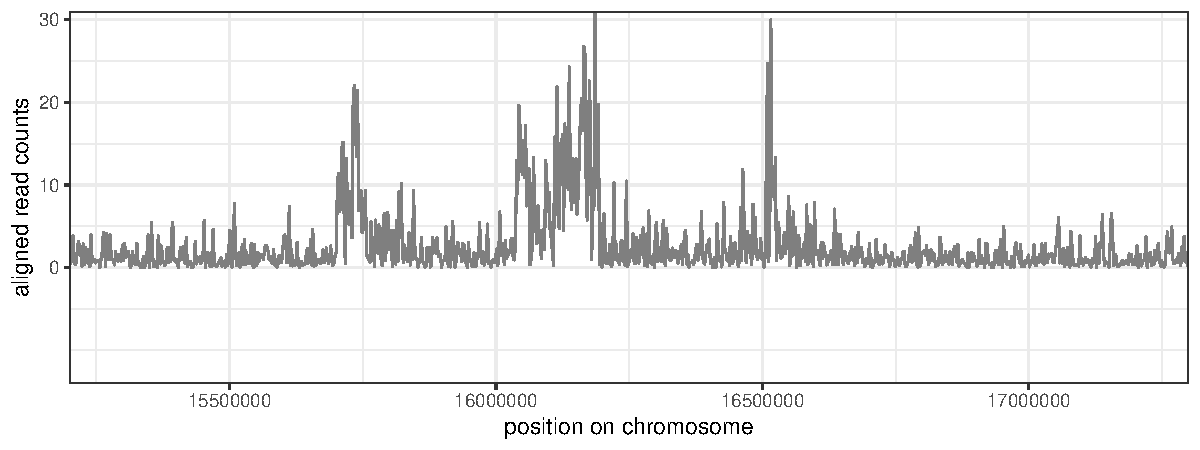
\includegraphics[width=\textwidth]{jss-figure-label-error-data}
  
  One ChIP-seq data set with $N=1,254,751$ (only 82,233 shown).
\end{frame}

\begin{frame}
  \frametitle{Labels used to determine optimal number of peaks}
  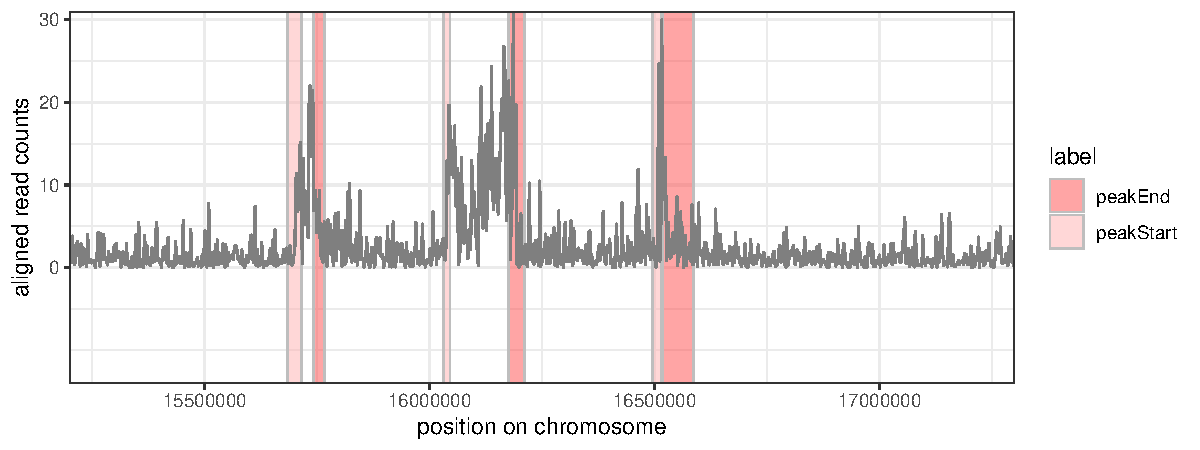
\includegraphics[width=\textwidth]{jss-figure-label-error-data-labels}

  Visually labeled regions (H {\it et al.}, {\it Bioinformatics} 2017). 
\end{frame}

\begin{frame}
  \frametitle{Labels used to determine optimal number of peaks}
  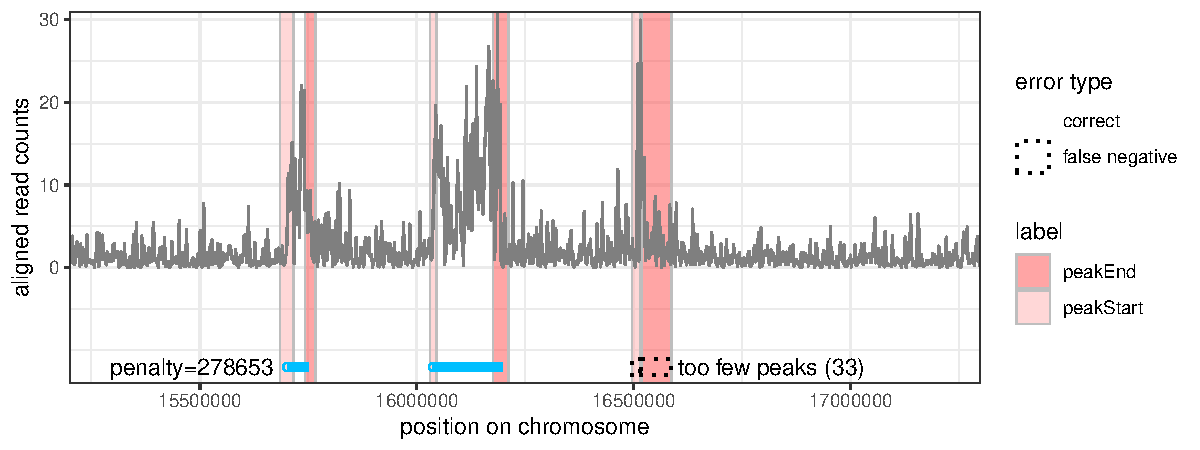
\includegraphics[width=\textwidth]{jss-figure-label-error-too-few}

  Penalty too large, too few peaks, 2 false negative labels.
\end{frame}

\begin{frame}
  \frametitle{Labels used to determine optimal number of peaks}
  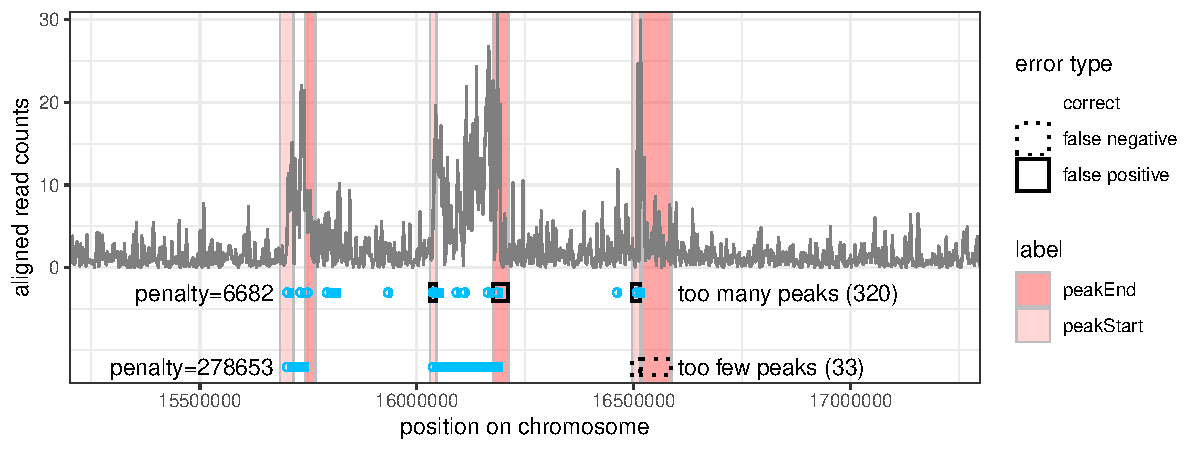
\includegraphics[width=\textwidth]{jss-figure-label-error-too-many}

  Penalty too small, too many peaks, 3 false positive labels.
\end{frame}

\begin{frame}
  \frametitle{Labels used to determine optimal number of peaks}
  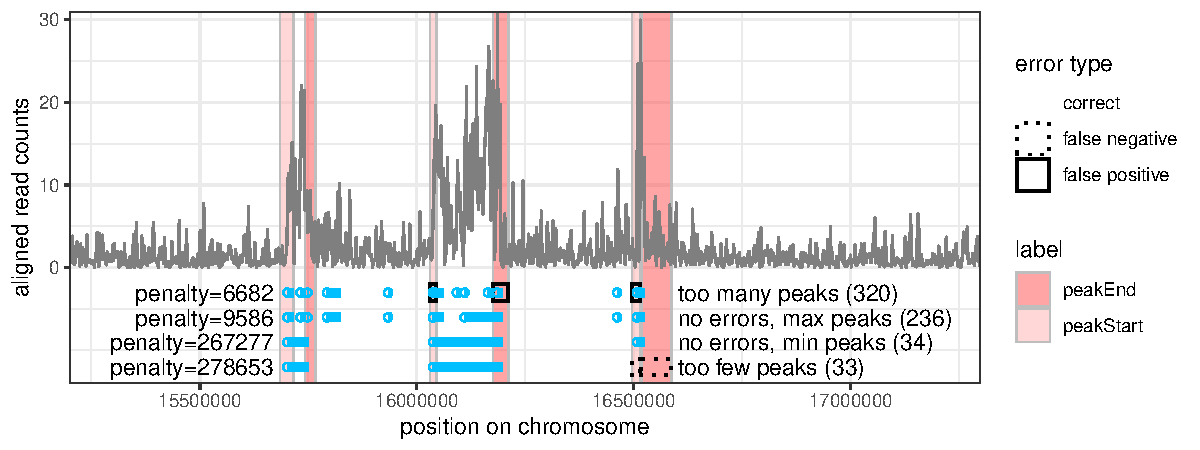
\includegraphics[width=\textwidth]{jss-figure-label-error}
   
  Models with 34--236 peaks have no label errors (midpoint=135).
\end{frame}  

\begin{frame}
  \frametitle{Segment Neighborhood model too slow for $O(\sqrt N)$ peaks }
  % Created by tikzDevice version 0.12.3.1 on 2021-08-27 10:42:22
% !TEX encoding = UTF-8 Unicode
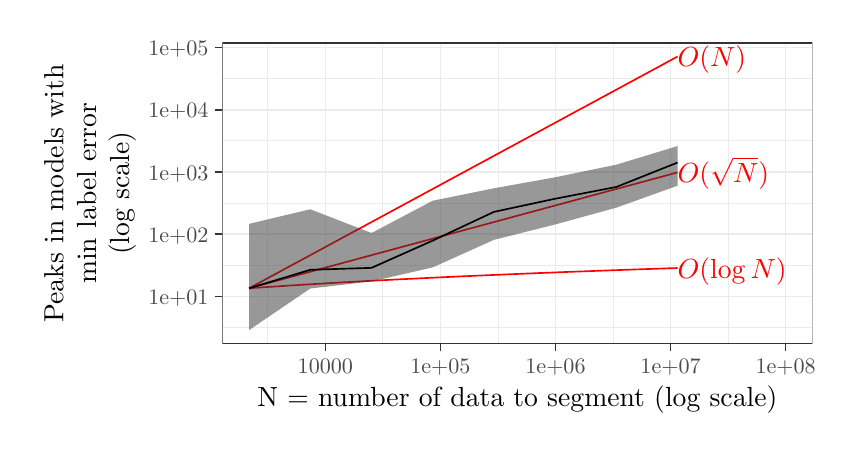
\begin{tikzpicture}[x=1pt,y=1pt]
\definecolor{fillColor}{RGB}{255,255,255}
\path[use as bounding box,fill=fillColor,fill opacity=0.00] (0,0) rectangle (289.08,144.54);
\begin{scope}
\path[clip] (  0.00,  0.00) rectangle (289.08,144.54);
\definecolor{drawColor}{RGB}{255,255,255}
\definecolor{fillColor}{RGB}{255,255,255}

\path[draw=drawColor,line width= 0.6pt,line join=round,line cap=round,fill=fillColor] (  0.00,  0.00) rectangle (289.08,144.54);
\end{scope}
\begin{scope}
\path[clip] ( 70.31, 30.33) rectangle (283.58,139.04);
\definecolor{fillColor}{RGB}{255,255,255}

\path[fill=fillColor] ( 70.31, 30.33) rectangle (283.58,139.04);
\definecolor{drawColor}{gray}{0.92}

\path[draw=drawColor,line width= 0.3pt,line join=round] ( 70.31, 36.20) --
	(283.58, 36.20);

\path[draw=drawColor,line width= 0.3pt,line join=round] ( 70.31, 58.68) --
	(283.58, 58.68);

\path[draw=drawColor,line width= 0.3pt,line join=round] ( 70.31, 81.17) --
	(283.58, 81.17);

\path[draw=drawColor,line width= 0.3pt,line join=round] ( 70.31,103.65) --
	(283.58,103.65);

\path[draw=drawColor,line width= 0.3pt,line join=round] ( 70.31,126.14) --
	(283.58,126.14);

\path[draw=drawColor,line width= 0.3pt,line join=round] ( 86.78, 30.33) --
	( 86.78,139.04);

\path[draw=drawColor,line width= 0.3pt,line join=round] (128.36, 30.33) --
	(128.36,139.04);

\path[draw=drawColor,line width= 0.3pt,line join=round] (169.94, 30.33) --
	(169.94,139.04);

\path[draw=drawColor,line width= 0.3pt,line join=round] (211.52, 30.33) --
	(211.52,139.04);

\path[draw=drawColor,line width= 0.3pt,line join=round] (253.10, 30.33) --
	(253.10,139.04);

\path[draw=drawColor,line width= 0.6pt,line join=round] ( 70.31, 47.44) --
	(283.58, 47.44);

\path[draw=drawColor,line width= 0.6pt,line join=round] ( 70.31, 69.93) --
	(283.58, 69.93);

\path[draw=drawColor,line width= 0.6pt,line join=round] ( 70.31, 92.41) --
	(283.58, 92.41);

\path[draw=drawColor,line width= 0.6pt,line join=round] ( 70.31,114.90) --
	(283.58,114.90);

\path[draw=drawColor,line width= 0.6pt,line join=round] ( 70.31,137.38) --
	(283.58,137.38);

\path[draw=drawColor,line width= 0.6pt,line join=round] (107.57, 30.33) --
	(107.57,139.04);

\path[draw=drawColor,line width= 0.6pt,line join=round] (149.15, 30.33) --
	(149.15,139.04);

\path[draw=drawColor,line width= 0.6pt,line join=round] (190.73, 30.33) --
	(190.73,139.04);

\path[draw=drawColor,line width= 0.6pt,line join=round] (232.31, 30.33) --
	(232.31,139.04);

\path[draw=drawColor,line width= 0.6pt,line join=round] (273.89, 30.33) --
	(273.89,139.04);
\definecolor{drawColor}{RGB}{255,0,0}

\path[draw=drawColor,line width= 0.6pt,line join=round] ( 80.01, 50.37) --
	( 81.57, 50.48) --
	( 83.13, 50.59) --
	( 84.70, 50.70) --
	( 86.26, 50.80) --
	( 87.82, 50.91) --
	( 89.39, 51.01) --
	( 90.95, 51.11) --
	( 92.52, 51.22) --
	( 94.08, 51.32) --
	( 95.64, 51.42) --
	( 97.21, 51.51) --
	( 98.77, 51.61) --
	(100.34, 51.71) --
	(101.90, 51.80) --
	(103.46, 51.90) --
	(105.03, 51.99) --
	(106.59, 52.08) --
	(108.16, 52.18) --
	(109.72, 52.27) --
	(111.28, 52.36) --
	(112.85, 52.45) --
	(114.41, 52.54) --
	(115.97, 52.62) --
	(117.54, 52.71) --
	(119.10, 52.80) --
	(120.67, 52.88) --
	(122.23, 52.97) --
	(123.79, 53.05) --
	(125.36, 53.13) --
	(126.92, 53.22) --
	(128.49, 53.30) --
	(130.05, 53.38) --
	(131.61, 53.46) --
	(133.18, 53.54) --
	(134.74, 53.62) --
	(136.31, 53.70) --
	(137.87, 53.78) --
	(139.43, 53.85) --
	(141.00, 53.93) --
	(142.56, 54.01) --
	(144.12, 54.08) --
	(145.69, 54.16) --
	(147.25, 54.23) --
	(148.82, 54.31) --
	(150.38, 54.38) --
	(151.94, 54.45) --
	(153.51, 54.52) --
	(155.07, 54.60) --
	(156.64, 54.67) --
	(158.20, 54.74) --
	(159.76, 54.81) --
	(161.33, 54.88) --
	(162.89, 54.95) --
	(164.46, 55.01) --
	(166.02, 55.08) --
	(167.58, 55.15) --
	(169.15, 55.22) --
	(170.71, 55.28) --
	(172.27, 55.35) --
	(173.84, 55.42) --
	(175.40, 55.48) --
	(176.97, 55.55) --
	(178.53, 55.61) --
	(180.09, 55.68) --
	(181.66, 55.74) --
	(183.22, 55.80) --
	(184.79, 55.87) --
	(186.35, 55.93) --
	(187.91, 55.99) --
	(189.48, 56.05) --
	(191.04, 56.11) --
	(192.61, 56.17) --
	(194.17, 56.24) --
	(195.73, 56.30) --
	(197.30, 56.36) --
	(198.86, 56.41) --
	(200.42, 56.47) --
	(201.99, 56.53) --
	(203.55, 56.59) --
	(205.12, 56.65) --
	(206.68, 56.71) --
	(208.24, 56.76) --
	(209.81, 56.82) --
	(211.37, 56.88) --
	(212.94, 56.93) --
	(214.50, 56.99) --
	(216.06, 57.05) --
	(217.63, 57.10) --
	(219.19, 57.16) --
	(220.76, 57.21) --
	(222.32, 57.27) --
	(223.88, 57.32) --
	(225.45, 57.37) --
	(227.01, 57.43) --
	(228.58, 57.48) --
	(230.14, 57.53) --
	(231.70, 57.59) --
	(233.27, 57.64) --
	(234.83, 57.69);

\path[draw=drawColor,line width= 0.6pt,line join=round] ( 80.01, 50.37) --
	( 81.57, 50.80) --
	( 83.13, 51.22) --
	( 84.70, 51.64) --
	( 86.26, 52.06) --
	( 87.82, 52.49) --
	( 89.39, 52.91) --
	( 90.95, 53.33) --
	( 92.52, 53.76) --
	( 94.08, 54.18) --
	( 95.64, 54.60) --
	( 97.21, 55.02) --
	( 98.77, 55.45) --
	(100.34, 55.87) --
	(101.90, 56.29) --
	(103.46, 56.72) --
	(105.03, 57.14) --
	(106.59, 57.56) --
	(108.16, 57.98) --
	(109.72, 58.41) --
	(111.28, 58.83) --
	(112.85, 59.25) --
	(114.41, 59.68) --
	(115.97, 60.10) --
	(117.54, 60.52) --
	(119.10, 60.94) --
	(120.67, 61.37) --
	(122.23, 61.79) --
	(123.79, 62.21) --
	(125.36, 62.64) --
	(126.92, 63.06) --
	(128.49, 63.48) --
	(130.05, 63.90) --
	(131.61, 64.33) --
	(133.18, 64.75) --
	(134.74, 65.17) --
	(136.31, 65.60) --
	(137.87, 66.02) --
	(139.43, 66.44) --
	(141.00, 66.86) --
	(142.56, 67.29) --
	(144.12, 67.71) --
	(145.69, 68.13) --
	(147.25, 68.56) --
	(148.82, 68.98) --
	(150.38, 69.40) --
	(151.94, 69.82) --
	(153.51, 70.25) --
	(155.07, 70.67) --
	(156.64, 71.09) --
	(158.20, 71.52) --
	(159.76, 71.94) --
	(161.33, 72.36) --
	(162.89, 72.78) --
	(164.46, 73.21) --
	(166.02, 73.63) --
	(167.58, 74.05) --
	(169.15, 74.48) --
	(170.71, 74.90) --
	(172.27, 75.32) --
	(173.84, 75.74) --
	(175.40, 76.17) --
	(176.97, 76.59) --
	(178.53, 77.01) --
	(180.09, 77.44) --
	(181.66, 77.86) --
	(183.22, 78.28) --
	(184.79, 78.70) --
	(186.35, 79.13) --
	(187.91, 79.55) --
	(189.48, 79.97) --
	(191.04, 80.40) --
	(192.61, 80.82) --
	(194.17, 81.24) --
	(195.73, 81.66) --
	(197.30, 82.09) --
	(198.86, 82.51) --
	(200.42, 82.93) --
	(201.99, 83.36) --
	(203.55, 83.78) --
	(205.12, 84.20) --
	(206.68, 84.62) --
	(208.24, 85.05) --
	(209.81, 85.47) --
	(211.37, 85.89) --
	(212.94, 86.32) --
	(214.50, 86.74) --
	(216.06, 87.16) --
	(217.63, 87.58) --
	(219.19, 88.01) --
	(220.76, 88.43) --
	(222.32, 88.85) --
	(223.88, 89.28) --
	(225.45, 89.70) --
	(227.01, 90.12) --
	(228.58, 90.54) --
	(230.14, 90.97) --
	(231.70, 91.39) --
	(233.27, 91.81) --
	(234.83, 92.24);

\path[draw=drawColor,line width= 0.6pt,line join=round] ( 80.01, 50.37) --
	( 81.57, 51.22) --
	( 83.13, 52.06) --
	( 84.70, 52.91) --
	( 86.26, 53.76) --
	( 87.82, 54.60) --
	( 89.39, 55.45) --
	( 90.95, 56.29) --
	( 92.52, 57.14) --
	( 94.08, 57.98) --
	( 95.64, 58.83) --
	( 97.21, 59.68) --
	( 98.77, 60.52) --
	(100.34, 61.37) --
	(101.90, 62.21) --
	(103.46, 63.06) --
	(105.03, 63.90) --
	(106.59, 64.75) --
	(108.16, 65.60) --
	(109.72, 66.44) --
	(111.28, 67.29) --
	(112.85, 68.13) --
	(114.41, 68.98) --
	(115.97, 69.82) --
	(117.54, 70.67) --
	(119.10, 71.52) --
	(120.67, 72.36) --
	(122.23, 73.21) --
	(123.79, 74.05) --
	(125.36, 74.90) --
	(126.92, 75.74) --
	(128.49, 76.59) --
	(130.05, 77.44) --
	(131.61, 78.28) --
	(133.18, 79.13) --
	(134.74, 79.97) --
	(136.31, 80.82) --
	(137.87, 81.66) --
	(139.43, 82.51) --
	(141.00, 83.36) --
	(142.56, 84.20) --
	(144.12, 85.05) --
	(145.69, 85.89) --
	(147.25, 86.74) --
	(148.82, 87.58) --
	(150.38, 88.43) --
	(151.94, 89.28) --
	(153.51, 90.12) --
	(155.07, 90.97) --
	(156.64, 91.81) --
	(158.20, 92.66) --
	(159.76, 93.50) --
	(161.33, 94.35) --
	(162.89, 95.20) --
	(164.46, 96.04) --
	(166.02, 96.89) --
	(167.58, 97.73) --
	(169.15, 98.58) --
	(170.71, 99.42) --
	(172.27,100.27) --
	(173.84,101.12) --
	(175.40,101.96) --
	(176.97,102.81) --
	(178.53,103.65) --
	(180.09,104.50) --
	(181.66,105.34) --
	(183.22,106.19) --
	(184.79,107.04) --
	(186.35,107.88) --
	(187.91,108.73) --
	(189.48,109.57) --
	(191.04,110.42) --
	(192.61,111.26) --
	(194.17,112.11) --
	(195.73,112.96) --
	(197.30,113.80) --
	(198.86,114.65) --
	(200.42,115.49) --
	(201.99,116.34) --
	(203.55,117.18) --
	(205.12,118.03) --
	(206.68,118.88) --
	(208.24,119.72) --
	(209.81,120.57) --
	(211.37,121.41) --
	(212.94,122.26) --
	(214.50,123.10) --
	(216.06,123.95) --
	(217.63,124.80) --
	(219.19,125.64) --
	(220.76,126.49) --
	(222.32,127.33) --
	(223.88,128.18) --
	(225.45,129.02) --
	(227.01,129.87) --
	(228.58,130.72) --
	(230.14,131.56) --
	(231.70,132.41) --
	(233.27,133.25) --
	(234.83,134.10);

\node[text=drawColor,anchor=base west,inner sep=0pt, outer sep=0pt, scale=  1.00] at (234.83,130.39) {$O(N)$};

\node[text=drawColor,anchor=base west,inner sep=0pt, outer sep=0pt, scale=  1.00] at (234.83, 53.98) {$O(\log N)$};

\node[text=drawColor,anchor=base west,inner sep=0pt, outer sep=0pt, scale=  1.00] at (234.83, 88.53) {$O(\sqrt N)$};
\definecolor{fillColor}{RGB}{51,51,51}

\path[fill=fillColor,fill opacity=0.50] ( 80.01, 73.65) --
	(102.12, 78.92) --
	(124.24, 70.34) --
	(146.36, 82.01) --
	(168.48, 86.50) --
	(190.59, 90.47) --
	(212.71, 95.03) --
	(234.83,101.75) --
	(234.83, 87.44) --
	(212.71, 79.50) --
	(190.59, 73.42) --
	(168.48, 67.87) --
	(146.36, 57.92) --
	(124.24, 52.84) --
	(102.12, 50.28) --
	( 80.01, 35.27) --
	cycle;

\path[] ( 80.01, 73.65) --
	(102.12, 78.92) --
	(124.24, 70.34) --
	(146.36, 82.01) --
	(168.48, 86.50) --
	(190.59, 90.47) --
	(212.71, 95.03) --
	(234.83,101.75);

\path[] (234.83, 87.44) --
	(212.71, 79.50) --
	(190.59, 73.42) --
	(168.48, 67.87) --
	(146.36, 57.92) --
	(124.24, 52.84) --
	(102.12, 50.28) --
	( 80.01, 35.27);
\definecolor{drawColor}{RGB}{0,0,0}

\path[draw=drawColor,line width= 0.6pt,line join=round] ( 80.01, 50.37) --
	(102.12, 57.05) --
	(124.24, 57.75) --
	(146.36, 67.59) --
	(168.48, 77.98) --
	(190.59, 82.72) --
	(212.71, 86.98) --
	(234.83, 95.80);
\definecolor{drawColor}{gray}{0.20}

\path[draw=drawColor,line width= 0.6pt,line join=round,line cap=round] ( 70.31, 30.33) rectangle (283.58,139.04);
\end{scope}
\begin{scope}
\path[clip] (  0.00,  0.00) rectangle (289.08,144.54);
\definecolor{drawColor}{gray}{0.30}

\node[text=drawColor,anchor=base east,inner sep=0pt, outer sep=0pt, scale=  0.80] at ( 65.36, 44.49) {1e+01};

\node[text=drawColor,anchor=base east,inner sep=0pt, outer sep=0pt, scale=  0.80] at ( 65.36, 66.97) {1e+02};

\node[text=drawColor,anchor=base east,inner sep=0pt, outer sep=0pt, scale=  0.80] at ( 65.36, 89.46) {1e+03};

\node[text=drawColor,anchor=base east,inner sep=0pt, outer sep=0pt, scale=  0.80] at ( 65.36,111.94) {1e+04};

\node[text=drawColor,anchor=base east,inner sep=0pt, outer sep=0pt, scale=  0.80] at ( 65.36,134.43) {1e+05};
\end{scope}
\begin{scope}
\path[clip] (  0.00,  0.00) rectangle (289.08,144.54);
\definecolor{drawColor}{gray}{0.20}

\path[draw=drawColor,line width= 0.6pt,line join=round] ( 67.56, 47.44) --
	( 70.31, 47.44);

\path[draw=drawColor,line width= 0.6pt,line join=round] ( 67.56, 69.93) --
	( 70.31, 69.93);

\path[draw=drawColor,line width= 0.6pt,line join=round] ( 67.56, 92.41) --
	( 70.31, 92.41);

\path[draw=drawColor,line width= 0.6pt,line join=round] ( 67.56,114.90) --
	( 70.31,114.90);

\path[draw=drawColor,line width= 0.6pt,line join=round] ( 67.56,137.38) --
	( 70.31,137.38);
\end{scope}
\begin{scope}
\path[clip] (  0.00,  0.00) rectangle (289.08,144.54);
\definecolor{drawColor}{gray}{0.20}

\path[draw=drawColor,line width= 0.6pt,line join=round] (107.57, 27.58) --
	(107.57, 30.33);

\path[draw=drawColor,line width= 0.6pt,line join=round] (149.15, 27.58) --
	(149.15, 30.33);

\path[draw=drawColor,line width= 0.6pt,line join=round] (190.73, 27.58) --
	(190.73, 30.33);

\path[draw=drawColor,line width= 0.6pt,line join=round] (232.31, 27.58) --
	(232.31, 30.33);

\path[draw=drawColor,line width= 0.6pt,line join=round] (273.89, 27.58) --
	(273.89, 30.33);
\end{scope}
\begin{scope}
\path[clip] (  0.00,  0.00) rectangle (289.08,144.54);
\definecolor{drawColor}{gray}{0.30}

\node[text=drawColor,anchor=base,inner sep=0pt, outer sep=0pt, scale=  0.80] at (107.57, 19.46) {10000};

\node[text=drawColor,anchor=base,inner sep=0pt, outer sep=0pt, scale=  0.80] at (149.15, 19.46) {1e+05};

\node[text=drawColor,anchor=base,inner sep=0pt, outer sep=0pt, scale=  0.80] at (190.73, 19.46) {1e+06};

\node[text=drawColor,anchor=base,inner sep=0pt, outer sep=0pt, scale=  0.80] at (232.31, 19.46) {1e+07};

\node[text=drawColor,anchor=base,inner sep=0pt, outer sep=0pt, scale=  0.80] at (273.89, 19.46) {1e+08};
\end{scope}
\begin{scope}
\path[clip] (  0.00,  0.00) rectangle (289.08,144.54);
\definecolor{drawColor}{RGB}{0,0,0}

\node[text=drawColor,anchor=base,inner sep=0pt, outer sep=0pt, scale=  1.00] at (176.95,  7.62) {N = number of data to segment (log scale)};
\end{scope}
\begin{scope}
\path[clip] (  0.00,  0.00) rectangle (289.08,144.54);
\definecolor{drawColor}{RGB}{0,0,0}

\node[text=drawColor,rotate= 90.00,anchor=base,inner sep=0pt, outer sep=0pt, scale=  1.00] at ( 12.89, 84.68) {Peaks in models with};

\node[text=drawColor,rotate= 90.00,anchor=base,inner sep=0pt, outer sep=0pt, scale=  1.00] at ( 24.77, 84.68) {min label error};

\node[text=drawColor,rotate= 90.00,anchor=base,inner sep=0pt, outer sep=0pt, scale=  1.00] at ( 36.65, 84.68) {(log scale)};
\end{scope}
\end{tikzpicture}

  \vskip -0.4cm
  \begin{itemize} 
  \item %H {\it et al.}, arXiv 2017: $O(SN\log N)$ time/space
    Previous GPDPA: $O(S)$ dynamic programming iterations,
    each is $O(N\log N)$ time/space.
  \item If we want $S=O(\sqrt{N})$ segments then the algorithm is
    $O(N \sqrt N \log N)$ time/space -- too much for large data.
  \item For example $N=10^7$ data. Each $O(N\log N)$ DP iteration
    takes 1 hour, 80 GB. Overall if we want $S=O(\sqrt N) = 2828$
    segments we need 220 TB of storage and 17 weeks!
  \end{itemize}
\end{frame}

\begin{frame}
  \frametitle{Implementation stores cost functions on disk}

  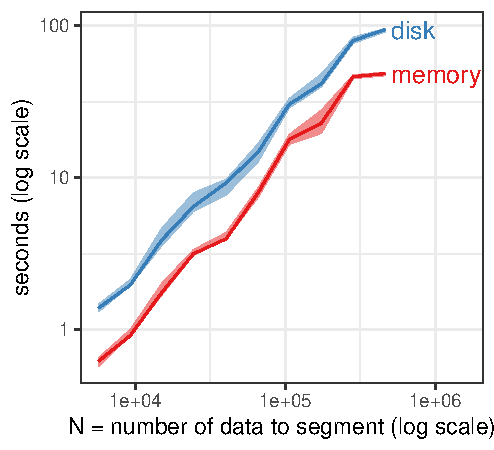
\includegraphics[width=0.5\textwidth]{jss-figure-disk-memory-compare-speed}

  \begin{itemize}
  \item Proposed GFPOP (Generalized FPOP) algorithm implemented using disk-based storage
    in R package \texttt{PeakSegDisk}.
  \item Disk storage is only a constant factor slower than memory.
  \item Both are $O(N\log N)$ time.
  \item Memory implementation: $O(N \log N)$ memory. (too big)
  \item Disk implementation: $O(\log N)$ memory ($<1$GB), $O(N\log N)$
    disk.
  \end{itemize}

\end{frame}

\begin{frame}[fragile]
  \frametitle{Time/space to solve one penalty is $O(N \log N)$}

  Total time/space = $O(NI)$ where $I$ is the number of intervals
  (candidate changepoints) stored in every optimal cost function.

  \begin{minipage}{0.48\textwidth}
\centering
    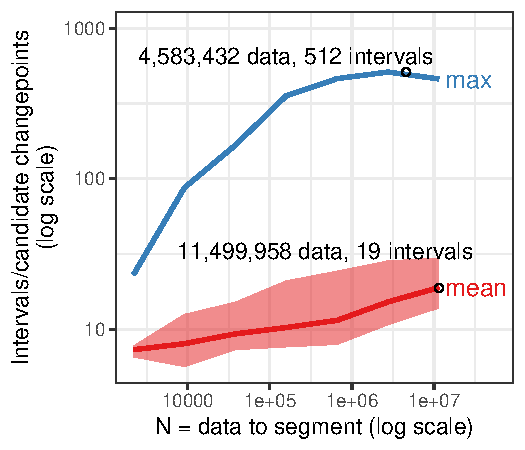
\includegraphics[width=\textwidth]{jss-figure-target-intervals-models}
    $I=O(\log N)$ intervals.
  \end{minipage}
  \begin{minipage}{0.48\textwidth}
\centering
    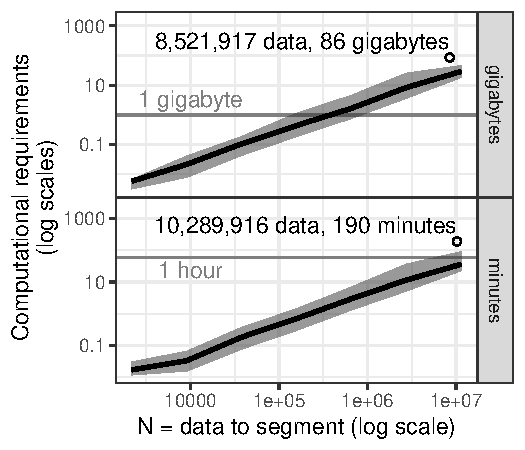
\includegraphics[width=\textwidth]{jss-figure-target-intervals-models-computation}
    Overall  $O(N \log N)$ complexity.
  \end{minipage}
  
\vskip 0.5cm
\begin{itemize}
\item So we can efficiently compute the best model for a given penalty
  $\lambda$.
\item But how to compute model with $O(\sqrt N)$ peaks?
\end{itemize}

\end{frame}

\begin{frame}
  \frametitle{Sequential search algorithm using GFPOP to compute most
    likely model with at most $P^*$ peaks}
  \begin{algorithmic}[1]
  \STATE Input: data $\mathbf z\in\RR^N$, target peaks $P^*$.
  \STATE $\overline L,\overline p \gets \text{GFPOP}(\mathbf z, \lambda=0)$ // max peak model
  \STATE $\underline L,\underline p \gets \text{GFPOP}(\mathbf z, \lambda=\infty)$ // 0 peak model
  \STATE While $\underline p\neq P^*$ and $\overline p\neq P^*$:
  \begin{ALC@g}
    \STATE \alert{$\lambda=(\overline L-\underline L)/(\underline p-\overline p)$}
    \STATE $L_{\text{new}},p_{\text{new}}\gets\text{GFPOP}(\mathbf z, \lambda)$
    \STATE If $p_{\text{new}}\in\{\underline p, \overline p\}$: return model with $\underline p$ peaks.
    \STATE If $p_{\text{new}} < P^*$: $\underline p\gets p_{\text{new}}$
    \STATE Else: $\overline p\gets p_{\text{new}}$
% > prob.i <- 3
% > fit.list$others[order(iteration)][, list(target.peaks=prob$peaks, iteration, under, over, penalty, peaks, total.cost)]
%    target.peaks iteration under over    penalty peaks total.cost
% 1:           33         1    NA   NA     0.0000  7487 -201361.96
% 2:           33         1    NA   NA        Inf     0  920923.98
% 3:           33         2     0 7487   149.8979   753  -24385.02
% 4:           33         3     0  753  1255.3904    47  153676.28
% 5:           33         4     0   47 16324.4191    10  310043.81
% 6:           33         5    10   47  4226.1495    21  214200.02
% 7:           33         6    21   47  2327.8360    33  177484.99
% > 
  \end{ALC@g}
  \STATE If $\underline p=P^*$: return model with $\underline p$ peaks.
  \STATE Else: return model with $\overline p$ peaks.
  \end{algorithmic}
\begin{itemize}
\item \alert{New penalty $\lambda$} guaranteed to make progress toward $P^*$ peaks.
\item Time complexity depends on number of iterations of while loop
  (number of calls to GFPOP sub-routine).
\end{itemize}
\end{frame}


\begin{frame}
  \frametitle{Example run of sequential search algorithm }
  \begin{itemize}
  \item One data set with $P^*=93$ peaks and $N=146,186$ data.
  \item 12 DP iterations much fewer than $93\times 2=186$ required for previous GPDPA (Segment Neighborhood problem).
  \end{itemize}
\small
  \begin{tabular}{rrrrrr}
 iteration& $\underline p$& $\overline p$&    $\lambda$ & $p_{\text{new}}$& $L_{\text{new}}$\\
\hline
         0&    &    &        $\infty$&     0&   14239212\\
         1&    &    &     0& 68752&   -2570319\\
         2&     0& 68752&   244.4952&  4361&    1980119\\
         3&     0&  4361&  2811.0738&   188&    3676671\\
         4&     0&   188& 56183.7271&    55&    5330310\\
         5&    55&   188& 12433.3766&    98&    4108354\\
         6&    55&    98& 28417.5941&    72&    4584042\\
         7&    72&    98& 18295.6895&    83&    4336773\\
         8&    83&    98& 15227.9249&    90&    4218815\\
         9&    90&    98& 13807.6282&    95&    4146172\\
        10&    90&    95& 14528.5052&    92&    4188881\\
        11&    92&    95& 14236.0863&    94&    4160179\\
        12&    92&    94& 14350.6622&    93&    4174480
  \end{tabular}

How large must the model size $P^*$ be for the new algorithm to be faster?

\end{frame}


\begin{frame}
  \frametitle{Only $O(\log N)$ runs of GFPOP even for large models}
  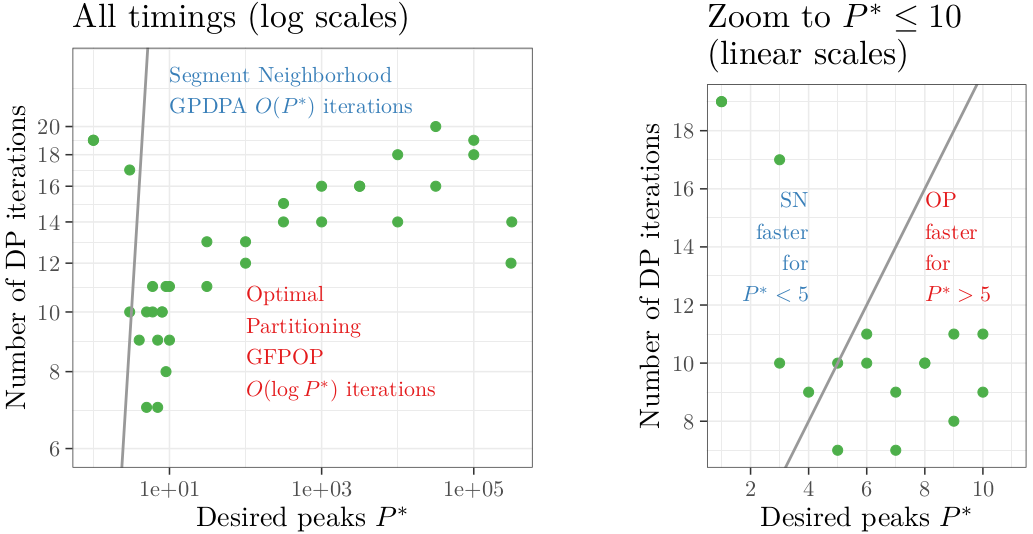
\includegraphics[width=\textwidth]{jss-figure-8}

  \begin{itemize}
  \item Experiment with two large data sequences $N\approx 10^7$,
    varying the number of desired peaks.
  \item Proposed Optimal Partitioning + sequential search
    algorithm is faster than previous Segment
    Neighborhood algorithm, for model sizes $P^*>5$.
  \end{itemize}
  
\end{frame}

\section{Conclusions}

\begin{frame}[fragile]
  \frametitle{Conclusion: optimal peak detection for large data}

  \begin{itemize}
  \item New algorithms for optimal changepoint detection in
    peak/background model, with constraints or penalty on number of
    changes/peaks.
  \item New R packages with efficient C++ code: PeakSegOptimal,
    PeakSegDisk.
  \item Makes it possible to compute an optimal model, with a large
    number of peaks, in huge genomic data sets, on your laptop.
  \item Future work: more general graph-based constraints for other
    data types (not just up-down peak pattern).
  \item Contact me: toby.hocking@nau.edu
  \item Thanks!
  \end{itemize}
  
\end{frame}

\begin{frame}
  \frametitle{For some data
 the desired number of peaks does not exist!}

One data set with $P^*=75$ and $N=66,031$ data.

\begin{tabular}{rrrrrr}
\small
 iteration& $\underline p$& $\overline p$&    $\lambda$ & $p_{\text{new}}$& $L_{\text{new}}$\\
  \hline
    1 &  &  & 0 & 29681 & -1495863.85 \\ 
    1 &  &  & $\infty$ &   0 & 1200631.42 \\ 
    2 &   0 & 29681 & 90.85 & 3445 & -1245181.37 \\ 
    3 &   0 & 3445 & 709.96 & 401 & -446632.57 \\ 
    4 &   0 & 401 & 4107.89 &  51 & 3105.03 \\ 
    5 &  51 & 401 & 1284.96 & 168 & -230152.31 \\ 
    6 &  51 & 168 & 1993.65 &  97 & -120725.83 \\ 
    7 &  51 &  97 & 2691.98 &  68 & -53946.18 \\ 
    8 &  68 &  97 & 2302.75 &  81 & -86423.80 \\ 
    9 &  68 &  81 & 2498.28 &  77 & -76891.10 \\ 
   10 &  68 &  77 & 2549.44 &  71 & -61722.09 \\ 
   11 &  71 &  77 & 2528.17 &  74 & -69330.62 \\ 
   12 &  74 &  77 & 2520.16 &  76 & -74374.78 \\ 
   13 &  \alert{74} &  \alert{76} & \alert{2522.08} &  \alert{76} & -74374.78 \\ 
\end{tabular}

\alert{No model exists between $\underline p=74$ and
  $\overline p=76$, so algo stops and returns the simpler model with 74 peaks.}

\end{frame}

\begin{frame}
  \frametitle{Number of GFPOP calls increases slowly with maximum number of peaks}
  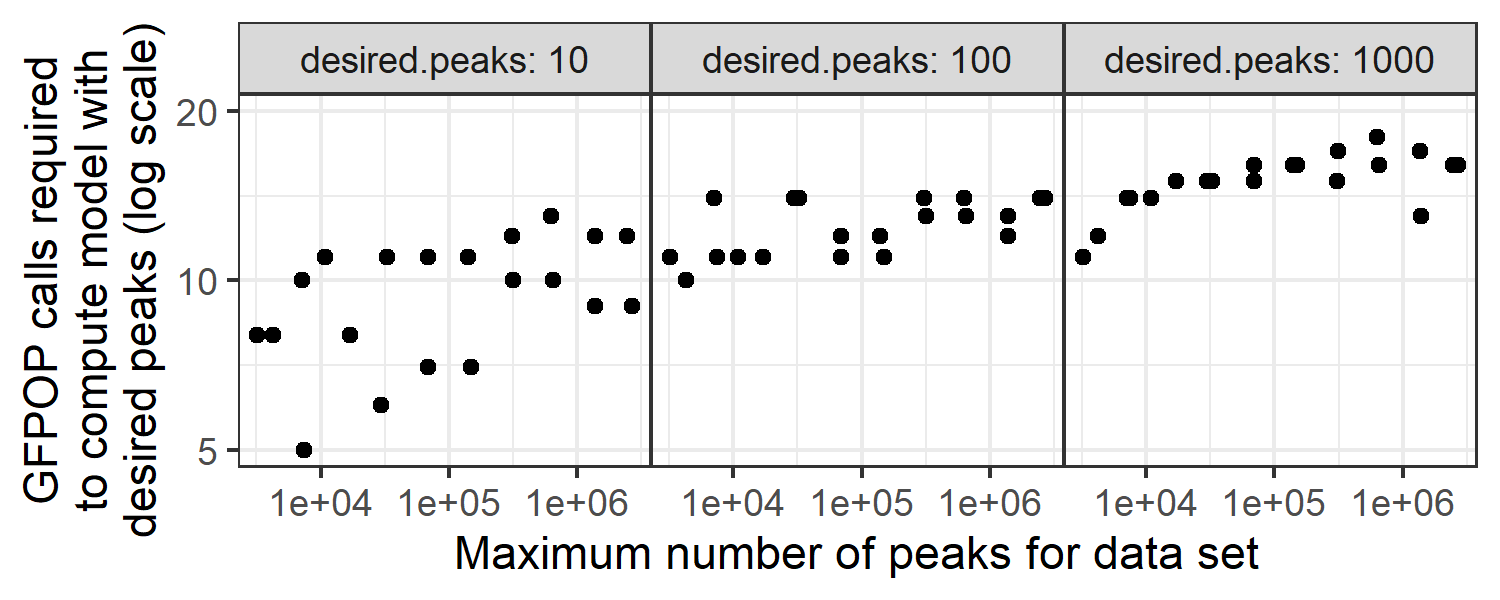
\includegraphics[width=\textwidth]{jss-figure-more-evals.png}
  \begin{itemize}
  \item Run GFPOP with penalty $\lambda=0$ to determine max number of
    peaks for each data sequence.
  \item Run sequential search on each data sequence with desired peaks
    $P^*\in\{10,100,1000\}$.
  \end{itemize}

\end{frame}

\begin{frame}
  \frametitle{Only $O(\log N)$ runs of GFPOP to compute $O(\sqrt N)$
    peaks}
  % Created by tikzDevice version 0.12.3.1 on 2021-08-27 11:08:28
% !TEX encoding = UTF-8 Unicode
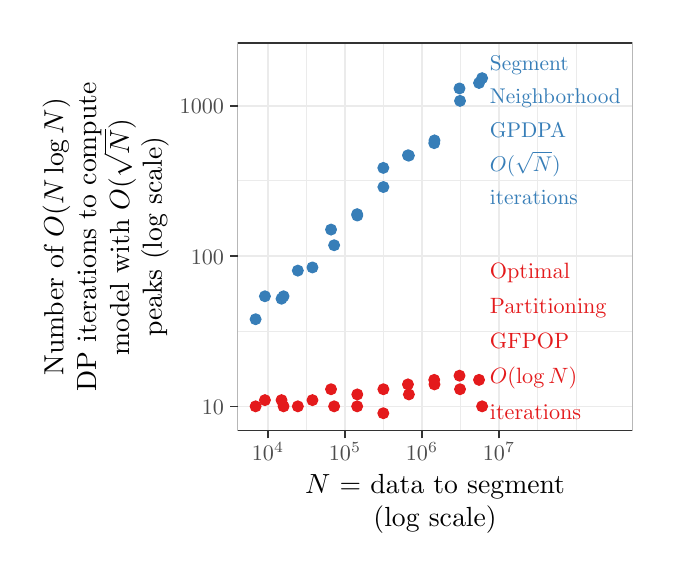
\begin{tikzpicture}[x=1pt,y=1pt]
\definecolor{fillColor}{RGB}{255,255,255}
\path[use as bounding box,fill=fillColor,fill opacity=0.00] (0,0) rectangle (224.04,187.90);
\begin{scope}
\path[clip] (  0.00,  0.00) rectangle (224.04,187.90);
\definecolor{drawColor}{RGB}{255,255,255}
\definecolor{fillColor}{RGB}{255,255,255}

\path[draw=drawColor,line width= 0.6pt,line join=round,line cap=round,fill=fillColor] (  0.00,  0.00) rectangle (224.04,187.90);
\end{scope}
\begin{scope}
\path[clip] ( 75.88, 42.21) rectangle (218.54,182.40);
\definecolor{fillColor}{RGB}{255,255,255}

\path[fill=fillColor] ( 75.88, 42.21) rectangle (218.54,182.40);
\definecolor{drawColor}{gray}{0.92}

\path[draw=drawColor,line width= 0.3pt,line join=round] ( 75.88, 78.22) --
	(218.54, 78.22);

\path[draw=drawColor,line width= 0.3pt,line join=round] ( 75.88,132.53) --
	(218.54,132.53);

\path[draw=drawColor,line width= 0.3pt,line join=round] (100.72, 42.21) --
	(100.72,182.40);

\path[draw=drawColor,line width= 0.3pt,line join=round] (128.56, 42.21) --
	(128.56,182.40);

\path[draw=drawColor,line width= 0.3pt,line join=round] (156.39, 42.21) --
	(156.39,182.40);

\path[draw=drawColor,line width= 0.3pt,line join=round] (184.22, 42.21) --
	(184.22,182.40);

\path[draw=drawColor,line width= 0.3pt,line join=round] (198.14, 42.21) --
	(198.14,182.40);

\path[draw=drawColor,line width= 0.6pt,line join=round] ( 75.88, 51.07) --
	(218.54, 51.07);

\path[draw=drawColor,line width= 0.6pt,line join=round] ( 75.88,105.37) --
	(218.54,105.37);

\path[draw=drawColor,line width= 0.6pt,line join=round] ( 75.88,159.68) --
	(218.54,159.68);

\path[draw=drawColor,line width= 0.6pt,line join=round] ( 86.81, 42.21) --
	( 86.81,182.40);

\path[draw=drawColor,line width= 0.6pt,line join=round] (114.64, 42.21) --
	(114.64,182.40);

\path[draw=drawColor,line width= 0.6pt,line join=round] (142.47, 42.21) --
	(142.47,182.40);

\path[draw=drawColor,line width= 0.6pt,line join=round] (170.30, 42.21) --
	(170.30,182.40);
\definecolor{drawColor}{RGB}{55,126,184}
\definecolor{fillColor}{RGB}{55,126,184}

\path[draw=drawColor,line width= 0.4pt,line join=round,line cap=round,fill=fillColor] ( 82.36, 82.55) circle (  1.96);

\path[draw=drawColor,line width= 0.4pt,line join=round,line cap=round,fill=fillColor] ( 85.73, 90.84) circle (  1.96);

\path[draw=drawColor,line width= 0.4pt,line join=round,line cap=round,fill=fillColor] ( 91.73, 89.95) circle (  1.96);

\path[draw=drawColor,line width= 0.4pt,line join=round,line cap=round,fill=fillColor] ( 92.46, 90.84) circle (  1.96);

\path[draw=drawColor,line width= 0.4pt,line join=round,line cap=round,fill=fillColor] ( 97.62,100.11) circle (  1.96);

\path[draw=drawColor,line width= 0.4pt,line join=round,line cap=round,fill=fillColor] (102.90,101.26) circle (  1.96);

\path[draw=drawColor,line width= 0.4pt,line join=round,line cap=round,fill=fillColor] (109.62,114.94) circle (  1.96);

\path[draw=drawColor,line width= 0.4pt,line join=round,line cap=round,fill=fillColor] (110.74,109.28) circle (  1.96);

\path[draw=drawColor,line width= 0.4pt,line join=round,line cap=round,fill=fillColor] (119.06,120.51) circle (  1.96);

\path[draw=drawColor,line width= 0.4pt,line join=round,line cap=round,fill=fillColor] (119.11,120.01) circle (  1.96);

\path[draw=drawColor,line width= 0.4pt,line join=round,line cap=round,fill=fillColor] (128.51,137.23) circle (  1.96);

\path[draw=drawColor,line width= 0.4pt,line join=round,line cap=round,fill=fillColor] (128.54,130.32) circle (  1.96);

\path[draw=drawColor,line width= 0.4pt,line join=round,line cap=round,fill=fillColor] (137.41,141.77) circle (  1.96);

\path[draw=drawColor,line width= 0.4pt,line join=round,line cap=round,fill=fillColor] (137.75,141.67) circle (  1.96);

\path[draw=drawColor,line width= 0.4pt,line join=round,line cap=round,fill=fillColor] (146.90,146.17) circle (  1.96);

\path[draw=drawColor,line width= 0.4pt,line join=round,line cap=round,fill=fillColor] (147.00,147.16) circle (  1.96);

\path[draw=drawColor,line width= 0.4pt,line join=round,line cap=round,fill=fillColor] (156.04,165.94) circle (  1.96);

\path[draw=drawColor,line width= 0.4pt,line join=round,line cap=round,fill=fillColor] (156.23,161.45) circle (  1.96);

\path[draw=drawColor,line width= 0.4pt,line join=round,line cap=round,fill=fillColor] (163.10,167.92) circle (  1.96);

\path[draw=drawColor,line width= 0.4pt,line join=round,line cap=round,fill=fillColor] (164.21,169.65) circle (  1.96);
\definecolor{drawColor}{RGB}{228,26,28}
\definecolor{fillColor}{RGB}{228,26,28}

\path[draw=drawColor,line width= 0.4pt,line join=round,line cap=round,fill=fillColor] ( 82.36, 51.07) circle (  1.96);

\path[draw=drawColor,line width= 0.4pt,line join=round,line cap=round,fill=fillColor] ( 85.73, 53.31) circle (  1.96);

\path[draw=drawColor,line width= 0.4pt,line join=round,line cap=round,fill=fillColor] ( 91.73, 53.31) circle (  1.96);

\path[draw=drawColor,line width= 0.4pt,line join=round,line cap=round,fill=fillColor] ( 92.46, 51.07) circle (  1.96);

\path[draw=drawColor,line width= 0.4pt,line join=round,line cap=round,fill=fillColor] ( 97.62, 51.07) circle (  1.96);

\path[draw=drawColor,line width= 0.4pt,line join=round,line cap=round,fill=fillColor] (102.90, 53.31) circle (  1.96);

\path[draw=drawColor,line width= 0.4pt,line join=round,line cap=round,fill=fillColor] (109.62, 57.25) circle (  1.96);

\path[draw=drawColor,line width= 0.4pt,line join=round,line cap=round,fill=fillColor] (110.74, 51.07) circle (  1.96);

\path[draw=drawColor,line width= 0.4pt,line join=round,line cap=round,fill=fillColor] (119.06, 51.07) circle (  1.96);

\path[draw=drawColor,line width= 0.4pt,line join=round,line cap=round,fill=fillColor] (119.11, 55.37) circle (  1.96);

\path[draw=drawColor,line width= 0.4pt,line join=round,line cap=round,fill=fillColor] (128.51, 48.58) circle (  1.96);

\path[draw=drawColor,line width= 0.4pt,line join=round,line cap=round,fill=fillColor] (128.54, 57.25) circle (  1.96);

\path[draw=drawColor,line width= 0.4pt,line join=round,line cap=round,fill=fillColor] (137.41, 59.00) circle (  1.96);

\path[draw=drawColor,line width= 0.4pt,line join=round,line cap=round,fill=fillColor] (137.75, 55.37) circle (  1.96);

\path[draw=drawColor,line width= 0.4pt,line join=round,line cap=round,fill=fillColor] (146.90, 60.63) circle (  1.96);

\path[draw=drawColor,line width= 0.4pt,line join=round,line cap=round,fill=fillColor] (147.00, 59.00) circle (  1.96);

\path[draw=drawColor,line width= 0.4pt,line join=round,line cap=round,fill=fillColor] (156.04, 62.15) circle (  1.96);

\path[draw=drawColor,line width= 0.4pt,line join=round,line cap=round,fill=fillColor] (156.23, 57.25) circle (  1.96);

\path[draw=drawColor,line width= 0.4pt,line join=round,line cap=round,fill=fillColor] (163.10, 60.63) circle (  1.96);

\path[draw=drawColor,line width= 0.4pt,line join=round,line cap=round,fill=fillColor] (164.21, 51.07) circle (  1.96);
\end{scope}
\begin{scope}
\path[clip] ( 75.88, 42.21) rectangle (218.54,182.40);
\definecolor{drawColor}{RGB}{228,26,28}

\node[text=drawColor,anchor=base west,inner sep=0pt, outer sep=0pt, scale=  0.80] at (167.05, 97.16) {Optimal};

\node[text=drawColor,anchor=base west,inner sep=0pt, outer sep=0pt, scale=  0.80] at (167.05, 84.49) {Partitioning};

\node[text=drawColor,anchor=base west,inner sep=0pt, outer sep=0pt, scale=  0.80] at (167.05, 71.82) {GFPOP};

\node[text=drawColor,anchor=base west,inner sep=0pt, outer sep=0pt, scale=  0.80] at (167.05, 59.15) {$O(\log N)$};

\node[text=drawColor,anchor=base west,inner sep=0pt, outer sep=0pt, scale=  0.80] at (167.05, 46.48) {iterations};
\definecolor{drawColor}{RGB}{55,126,184}

\node[text=drawColor,anchor=base west,inner sep=0pt, outer sep=0pt, scale=  0.77] at (167.05,172.47) {Segment};

\node[text=drawColor,anchor=base west,inner sep=0pt, outer sep=0pt, scale=  0.77] at (167.05,160.33) {Neighborhood};

\node[text=drawColor,anchor=base west,inner sep=0pt, outer sep=0pt, scale=  0.77] at (167.05,148.19) {GPDPA};

\node[text=drawColor,anchor=base west,inner sep=0pt, outer sep=0pt, scale=  0.77] at (167.05,136.06) {$O(\sqrt N)$};

\node[text=drawColor,anchor=base west,inner sep=0pt, outer sep=0pt, scale=  0.77] at (167.05,123.92) {iterations};
\definecolor{drawColor}{gray}{0.20}

\path[draw=drawColor,line width= 0.6pt,line join=round,line cap=round] ( 75.88, 42.21) rectangle (218.54,182.40);
\end{scope}
\begin{scope}
\path[clip] (  0.00,  0.00) rectangle (224.04,187.90);
\definecolor{drawColor}{gray}{0.30}

\node[text=drawColor,anchor=base east,inner sep=0pt, outer sep=0pt, scale=  0.80] at ( 70.93, 48.11) {10};

\node[text=drawColor,anchor=base east,inner sep=0pt, outer sep=0pt, scale=  0.80] at ( 70.93,102.42) {100};

\node[text=drawColor,anchor=base east,inner sep=0pt, outer sep=0pt, scale=  0.80] at ( 70.93,156.72) {1000};
\end{scope}
\begin{scope}
\path[clip] (  0.00,  0.00) rectangle (224.04,187.90);
\definecolor{drawColor}{gray}{0.20}

\path[draw=drawColor,line width= 0.6pt,line join=round] ( 73.13, 51.07) --
	( 75.88, 51.07);

\path[draw=drawColor,line width= 0.6pt,line join=round] ( 73.13,105.37) --
	( 75.88,105.37);

\path[draw=drawColor,line width= 0.6pt,line join=round] ( 73.13,159.68) --
	( 75.88,159.68);
\end{scope}
\begin{scope}
\path[clip] (  0.00,  0.00) rectangle (224.04,187.90);
\definecolor{drawColor}{gray}{0.20}

\path[draw=drawColor,line width= 0.6pt,line join=round] ( 86.81, 39.46) --
	( 86.81, 42.21);

\path[draw=drawColor,line width= 0.6pt,line join=round] (114.64, 39.46) --
	(114.64, 42.21);

\path[draw=drawColor,line width= 0.6pt,line join=round] (142.47, 39.46) --
	(142.47, 42.21);

\path[draw=drawColor,line width= 0.6pt,line join=round] (170.30, 39.46) --
	(170.30, 42.21);
\end{scope}
\begin{scope}
\path[clip] (  0.00,  0.00) rectangle (224.04,187.90);
\definecolor{drawColor}{gray}{0.30}

\node[text=drawColor,anchor=base,inner sep=0pt, outer sep=0pt, scale=  0.80] at ( 86.81, 31.34) {$10^4$};

\node[text=drawColor,anchor=base,inner sep=0pt, outer sep=0pt, scale=  0.80] at (114.64, 31.34) {$10^5$};

\node[text=drawColor,anchor=base,inner sep=0pt, outer sep=0pt, scale=  0.80] at (142.47, 31.34) {$10^6$};

\node[text=drawColor,anchor=base,inner sep=0pt, outer sep=0pt, scale=  0.80] at (170.30, 31.34) {$10^7$};
\end{scope}
\begin{scope}
\path[clip] (  0.00,  0.00) rectangle (224.04,187.90);
\definecolor{drawColor}{RGB}{0,0,0}

\node[text=drawColor,anchor=base,inner sep=0pt, outer sep=0pt, scale=  1.00] at (147.21, 19.50) {$N$ = data to segment};

\node[text=drawColor,anchor=base,inner sep=0pt, outer sep=0pt, scale=  1.00] at (147.21,  7.62) {(log scale)};
\end{scope}
\begin{scope}
\path[clip] (  0.00,  0.00) rectangle (224.04,187.90);
\definecolor{drawColor}{RGB}{0,0,0}

\node[text=drawColor,rotate= 90.00,anchor=base,inner sep=0pt, outer sep=0pt, scale=  1.00] at ( 12.89,112.30) {Number of $O(N \log N)$};

\node[text=drawColor,rotate= 90.00,anchor=base,inner sep=0pt, outer sep=0pt, scale=  1.00] at ( 24.77,112.30) {DP iterations to compute};

\node[text=drawColor,rotate= 90.00,anchor=base,inner sep=0pt, outer sep=0pt, scale=  1.00] at ( 36.65,112.30) {model with $O(\sqrt N)$};

\node[text=drawColor,rotate= 90.00,anchor=base,inner sep=0pt, outer sep=0pt, scale=  1.00] at ( 48.53,112.30) {peaks (log scale)};
\end{scope}
\end{tikzpicture}


  \begin{itemize}
  \item Proposed Optimal Partitioning algorithm + sequential search
    algorithm is much faster than previous Segment
    Neighborhood algorithm. 
  \end{itemize}
  
\end{frame}

\begin{frame}
  \frametitle{Sequential search only a log factor slower than solving one penalty}
  % Created by tikzDevice version 0.12.3 on 2020-01-08 13:36:11
% !TEX encoding = UTF-8 Unicode
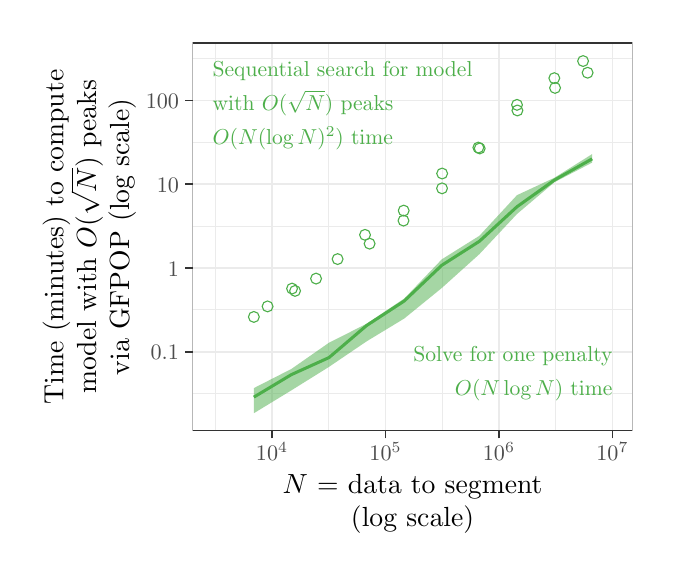
\begin{tikzpicture}[x=1pt,y=1pt]
\definecolor{fillColor}{RGB}{255,255,255}
\path[use as bounding box,fill=fillColor,fill opacity=0.00] (0,0) rectangle (224.04,187.90);
\begin{scope}
\path[clip] (  0.00,  0.00) rectangle (224.04,187.90);
\definecolor{drawColor}{RGB}{255,255,255}
\definecolor{fillColor}{RGB}{255,255,255}

\path[draw=drawColor,line width= 0.6pt,line join=round,line cap=round,fill=fillColor] (  0.00,  0.00) rectangle (224.04,187.90);
\end{scope}
\begin{scope}
\path[clip] ( 59.62, 42.21) rectangle (218.54,182.40);
\definecolor{fillColor}{RGB}{255,255,255}

\path[fill=fillColor] ( 59.62, 42.21) rectangle (218.54,182.40);
\definecolor{drawColor}{gray}{0.92}

\path[draw=drawColor,line width= 0.3pt,line join=round] ( 59.62, 55.66) --
	(218.54, 55.66);

\path[draw=drawColor,line width= 0.3pt,line join=round] ( 59.62, 85.93) --
	(218.54, 85.93);

\path[draw=drawColor,line width= 0.3pt,line join=round] ( 59.62,116.19) --
	(218.54,116.19);

\path[draw=drawColor,line width= 0.3pt,line join=round] ( 59.62,146.46) --
	(218.54,146.46);

\path[draw=drawColor,line width= 0.3pt,line join=round] ( 59.62,176.72) --
	(218.54,176.72);

\path[draw=drawColor,line width= 0.3pt,line join=round] ( 67.78, 42.21) --
	( 67.78,182.40);

\path[draw=drawColor,line width= 0.3pt,line join=round] (108.79, 42.21) --
	(108.79,182.40);

\path[draw=drawColor,line width= 0.3pt,line join=round] (149.80, 42.21) --
	(149.80,182.40);

\path[draw=drawColor,line width= 0.3pt,line join=round] (190.81, 42.21) --
	(190.81,182.40);

\path[draw=drawColor,line width= 0.6pt,line join=round] ( 59.62, 70.79) --
	(218.54, 70.79);

\path[draw=drawColor,line width= 0.6pt,line join=round] ( 59.62,101.06) --
	(218.54,101.06);

\path[draw=drawColor,line width= 0.6pt,line join=round] ( 59.62,131.32) --
	(218.54,131.32);

\path[draw=drawColor,line width= 0.6pt,line join=round] ( 59.62,161.59) --
	(218.54,161.59);

\path[draw=drawColor,line width= 0.6pt,line join=round] ( 88.28, 42.21) --
	( 88.28,182.40);

\path[draw=drawColor,line width= 0.6pt,line join=round] (129.29, 42.21) --
	(129.29,182.40);

\path[draw=drawColor,line width= 0.6pt,line join=round] (170.30, 42.21) --
	(170.30,182.40);

\path[draw=drawColor,line width= 0.6pt,line join=round] (211.31, 42.21) --
	(211.31,182.40);
\definecolor{drawColor}{RGB}{77,175,74}

\node[text=drawColor,anchor=base west,inner sep=0pt, outer sep=0pt, scale=  0.78] at ( 66.84,170.29) {Sequential search for model};

\node[text=drawColor,anchor=base west,inner sep=0pt, outer sep=0pt, scale=  0.78] at ( 66.84,158.00) {with $O(\sqrt N)$ peaks};

\node[text=drawColor,anchor=base west,inner sep=0pt, outer sep=0pt, scale=  0.78] at ( 66.84,145.71) {$O(N(\log N)^2)$ time};

\node[text=drawColor,anchor=base east,inner sep=0pt, outer sep=0pt, scale=  0.78] at (211.31, 67.26) {Solve for one penalty};

\node[text=drawColor,anchor=base east,inner sep=0pt, outer sep=0pt, scale=  0.78] at (211.31, 54.97) {$O(N \log N)$ time};
\definecolor{fillColor}{RGB}{77,175,74}

\path[fill=fillColor,fill opacity=0.50] ( 81.73, 57.66) --
	( 95.31, 64.59) --
	(108.89, 74.06) --
	(122.47, 80.91) --
	(136.06, 90.01) --
	(149.64,104.19) --
	(163.22,112.69) --
	(176.80,127.37) --
	(190.38,133.69) --
	(203.97,142.22) --
	(203.97,139.13) --
	(190.38,132.07) --
	(176.80,120.56) --
	(163.22,106.05) --
	(149.64, 93.83) --
	(136.06, 82.79) --
	(122.47, 74.55) --
	(108.89, 65.34) --
	( 95.31, 56.86) --
	( 81.73, 48.58) --
	cycle;

\path[draw=drawColor,line width= 1.1pt,line join=round] ( 81.73, 54.40) --
	( 95.31, 62.54) --
	(108.89, 68.69) --
	(122.47, 80.27) --
	(136.06, 89.12) --
	(149.64,102.04) --
	(163.22,110.70) --
	(176.80,123.18) --
	(190.38,132.86) --
	(203.97,140.50);

\path[draw=drawColor,line width= 0.4pt,line join=round,line cap=round] ( 81.73, 83.38) circle (  1.96);

\path[draw=drawColor,line width= 0.4pt,line join=round,line cap=round] ( 86.69, 87.18) circle (  1.96);

\path[draw=drawColor,line width= 0.4pt,line join=round,line cap=round] ( 95.53, 93.62) circle (  1.96);

\path[draw=drawColor,line width= 0.4pt,line join=round,line cap=round] ( 96.62, 92.78) circle (  1.96);

\path[draw=drawColor,line width= 0.4pt,line join=round,line cap=round] (104.21, 97.23) circle (  1.96);

\path[draw=drawColor,line width= 0.4pt,line join=round,line cap=round] (111.99,104.28) circle (  1.96);

\path[draw=drawColor,line width= 0.4pt,line join=round,line cap=round] (121.90,113.04) circle (  1.96);

\path[draw=drawColor,line width= 0.4pt,line join=round,line cap=round] (123.55,109.85) circle (  1.96);

\path[draw=drawColor,line width= 0.4pt,line join=round,line cap=round] (135.80,118.18) circle (  1.96);

\path[draw=drawColor,line width= 0.4pt,line join=round,line cap=round] (135.87,121.80) circle (  1.96);

\path[draw=drawColor,line width= 0.4pt,line join=round,line cap=round] (149.73,129.84) circle (  1.96);

\path[draw=drawColor,line width= 0.4pt,line join=round,line cap=round] (149.77,135.20) circle (  1.96);

\path[draw=drawColor,line width= 0.4pt,line join=round,line cap=round] (162.85,144.58) circle (  1.96);

\path[draw=drawColor,line width= 0.4pt,line join=round,line cap=round] (163.34,144.25) circle (  1.96);

\path[draw=drawColor,line width= 0.4pt,line join=round,line cap=round] (176.82,160.01) circle (  1.96);

\path[draw=drawColor,line width= 0.4pt,line join=round,line cap=round] (176.97,157.98) circle (  1.96);

\path[draw=drawColor,line width= 0.4pt,line join=round,line cap=round] (190.30,169.66) circle (  1.96);

\path[draw=drawColor,line width= 0.4pt,line join=round,line cap=round] (190.57,166.13) circle (  1.96);

\path[draw=drawColor,line width= 0.4pt,line join=round,line cap=round] (200.69,175.84) circle (  1.96);

\path[draw=drawColor,line width= 0.4pt,line join=round,line cap=round] (202.33,171.62) circle (  1.96);
\definecolor{drawColor}{gray}{0.20}

\path[draw=drawColor,line width= 0.6pt,line join=round,line cap=round] ( 59.62, 42.21) rectangle (218.54,182.40);
\end{scope}
\begin{scope}
\path[clip] (  0.00,  0.00) rectangle (224.04,187.90);
\definecolor{drawColor}{gray}{0.30}

\node[text=drawColor,anchor=base east,inner sep=0pt, outer sep=0pt, scale=  0.80] at ( 54.67, 67.84) {0.1};

\node[text=drawColor,anchor=base east,inner sep=0pt, outer sep=0pt, scale=  0.80] at ( 54.67, 98.10) {1};

\node[text=drawColor,anchor=base east,inner sep=0pt, outer sep=0pt, scale=  0.80] at ( 54.67,128.37) {10};

\node[text=drawColor,anchor=base east,inner sep=0pt, outer sep=0pt, scale=  0.80] at ( 54.67,158.63) {100};
\end{scope}
\begin{scope}
\path[clip] (  0.00,  0.00) rectangle (224.04,187.90);
\definecolor{drawColor}{gray}{0.20}

\path[draw=drawColor,line width= 0.6pt,line join=round] ( 56.87, 70.79) --
	( 59.62, 70.79);

\path[draw=drawColor,line width= 0.6pt,line join=round] ( 56.87,101.06) --
	( 59.62,101.06);

\path[draw=drawColor,line width= 0.6pt,line join=round] ( 56.87,131.32) --
	( 59.62,131.32);

\path[draw=drawColor,line width= 0.6pt,line join=round] ( 56.87,161.59) --
	( 59.62,161.59);
\end{scope}
\begin{scope}
\path[clip] (  0.00,  0.00) rectangle (224.04,187.90);
\definecolor{drawColor}{gray}{0.20}

\path[draw=drawColor,line width= 0.6pt,line join=round] ( 88.28, 39.46) --
	( 88.28, 42.21);

\path[draw=drawColor,line width= 0.6pt,line join=round] (129.29, 39.46) --
	(129.29, 42.21);

\path[draw=drawColor,line width= 0.6pt,line join=round] (170.30, 39.46) --
	(170.30, 42.21);

\path[draw=drawColor,line width= 0.6pt,line join=round] (211.31, 39.46) --
	(211.31, 42.21);
\end{scope}
\begin{scope}
\path[clip] (  0.00,  0.00) rectangle (224.04,187.90);
\definecolor{drawColor}{gray}{0.30}

\node[text=drawColor,anchor=base,inner sep=0pt, outer sep=0pt, scale=  0.80] at ( 88.28, 31.34) {$10^4$};

\node[text=drawColor,anchor=base,inner sep=0pt, outer sep=0pt, scale=  0.80] at (129.29, 31.34) {$10^5$};

\node[text=drawColor,anchor=base,inner sep=0pt, outer sep=0pt, scale=  0.80] at (170.30, 31.34) {$10^6$};

\node[text=drawColor,anchor=base,inner sep=0pt, outer sep=0pt, scale=  0.80] at (211.31, 31.34) {$10^7$};
\end{scope}
\begin{scope}
\path[clip] (  0.00,  0.00) rectangle (224.04,187.90);
\definecolor{drawColor}{RGB}{0,0,0}

\node[text=drawColor,anchor=base,inner sep=0pt, outer sep=0pt, scale=  1.00] at (139.08, 19.50) {$N$ = data to segment};

\node[text=drawColor,anchor=base,inner sep=0pt, outer sep=0pt, scale=  1.00] at (139.08,  7.62) {(log scale)};
\end{scope}
\begin{scope}
\path[clip] (  0.00,  0.00) rectangle (224.04,187.90);
\definecolor{drawColor}{RGB}{0,0,0}

\node[text=drawColor,rotate= 90.00,anchor=base,inner sep=0pt, outer sep=0pt, scale=  1.00] at ( 12.89,112.30) {Time (minutes) to compute};

\node[text=drawColor,rotate= 90.00,anchor=base,inner sep=0pt, outer sep=0pt, scale=  1.00] at ( 24.77,112.30) {     model with $O(\sqrt N)$ peaks};

\node[text=drawColor,rotate= 90.00,anchor=base,inner sep=0pt, outer sep=0pt, scale=  1.00] at ( 36.65,112.30) {     via GFPOP (log scale)};
\end{scope}
\end{tikzpicture}
 

  For $N=10^7$ only several hours of computation! (compare with weeks
  for Segment Neighborhood algorithm)
  
\end{frame}

\begin{frame}
  \frametitle{Chromatin immunoprecipitation sequencing (ChIP-seq)}
  Analysis of DNA-protein interactions.

  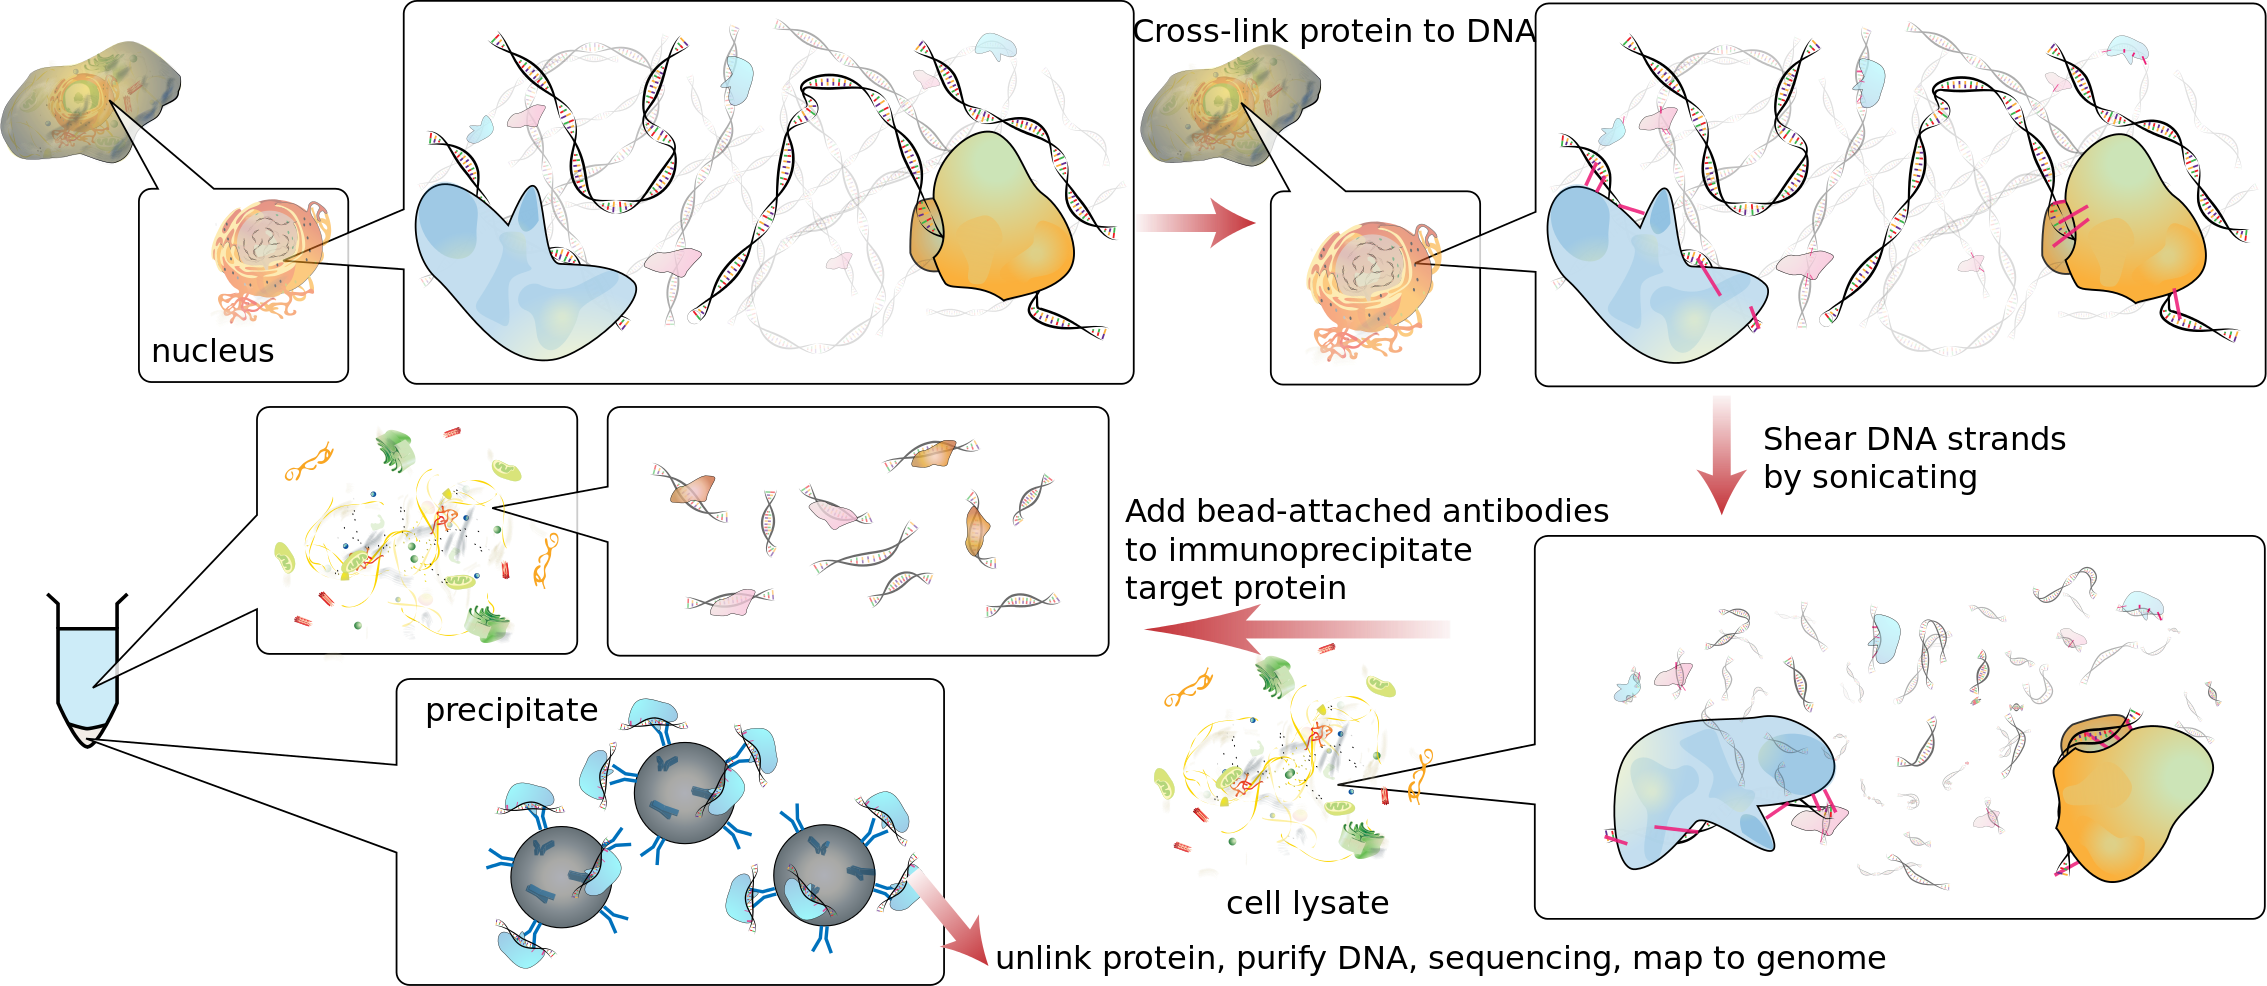
\includegraphics[width=\textwidth]{Chromatin_immunoprecipitation_sequencing_wide.png}

  Source: ``ChIP-sequencing,'' Wikipedia.
\end{frame}

% \begin{frame}
%   \frametitle{Previous work in genomic peak detection}
%   \begin{itemize}
%   \item Model-based analysis of ChIP-Seq (MACS), Zhang et al, 2008.
%   \item SICER, Zang et al, 2009.
%   \item HOMER, Heinz et al, 2010.
%   \item CCAT, Xu et al, 2010.
%   \item RSEG, Song et al, 2011.
%   \item Triform, Kornacker et al, 2012.
%   \item Histone modifications in cancer (HMCan), Ashoor et al, 2013.
%   \item PeakSeg, Hocking, Rigaill, Bourque, ICML 2015.
%   %\item PeakSegJoint Hocking and Bourque, arXiv:1506.01286.
%   \item ... dozens of others.
%   \end{itemize}
%   Two big questions: how to choose the best...
%   \begin{itemize}
%   \item ...algorithm? (testing)
%   \item \alert<1>{...parameters? (training)}
%   \end{itemize}
% \end{frame}

% \begin{frame}[fragile]
%   \frametitle{How to choose parameters of unsupervised peak
%     detectors?}
% \scriptsize
% 19 parameters for Model-based analysis of ChIP-Seq (MACS), Zhang et al, 2008.
% \begin{verbatim}
%   [-g GSIZE]
%   [-s TSIZE] [--bw BW] [-m MFOLD MFOLD] [--fix-bimodal]
%   [--nomodel] [--extsize EXTSIZE | --shiftsize SHIFTSIZE]
%   [-q QVALUE | -p PVALUE | -F FOLDENRICHMENT] [--to-large]
%   [--down-sample] [--seed SEED] [--nolambda]
%   [--slocal SMALLLOCAL] [--llocal LARGELOCAL]
%   [--shift-control] [--half-ext] [--broad]
%   [--broad-cutoff BROADCUTOFF] [--call-summits]
% \end{verbatim}
% 10 parameters for Histone modifications in cancer (HMCan),
% Ashoor et al, 2013.
% \begin{verbatim}
% minLength 145
% medLength 150
% maxLength 155
% smallBinLength 50
% largeBinLength 100000
% pvalueThreshold 0.01
% mergeDistance 200
% iterationThreshold 5
% finalThreshold 0
% maxIter 20
% \end{verbatim}
% \end{frame}
 
\begin{frame}
  \frametitle{Which macs parameter is best for these data?}
  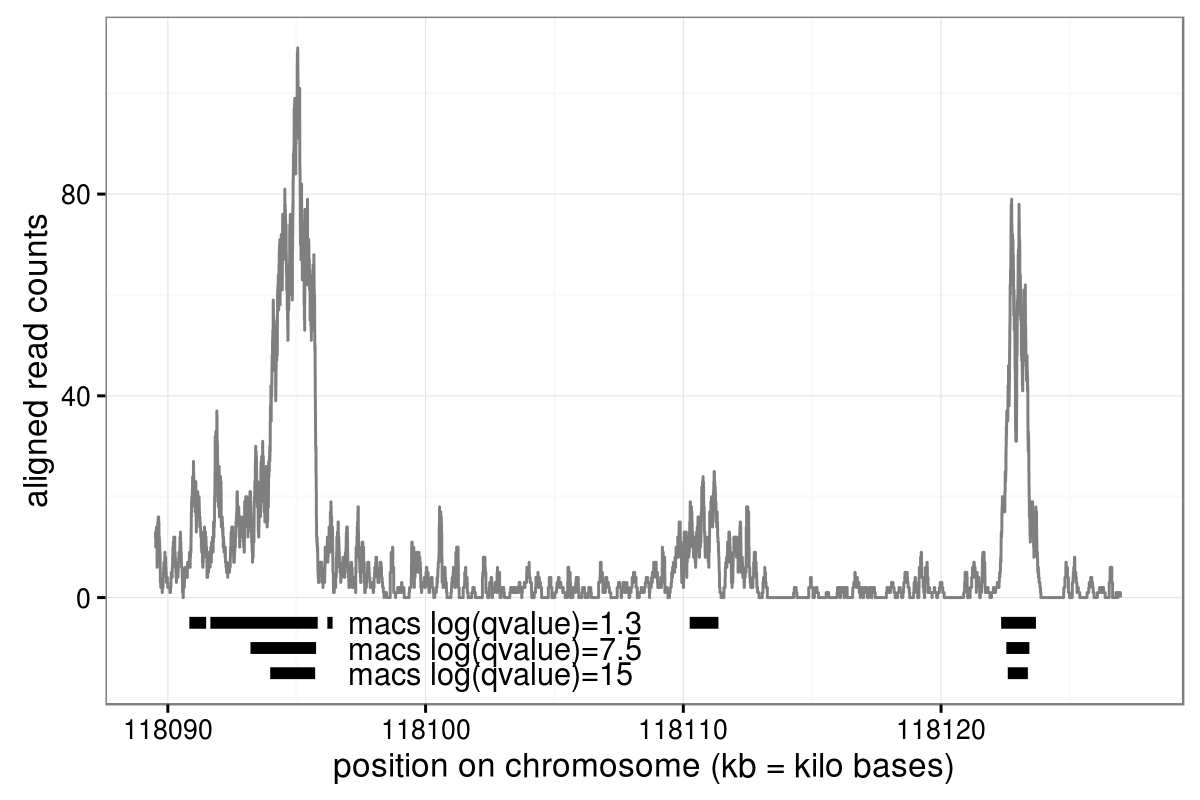
\includegraphics[width=1\textwidth]{figure-macs-problem.png}
\end{frame}

\begin{frame}
  \frametitle{Compute likelihood/loss of piecewise constant model}
  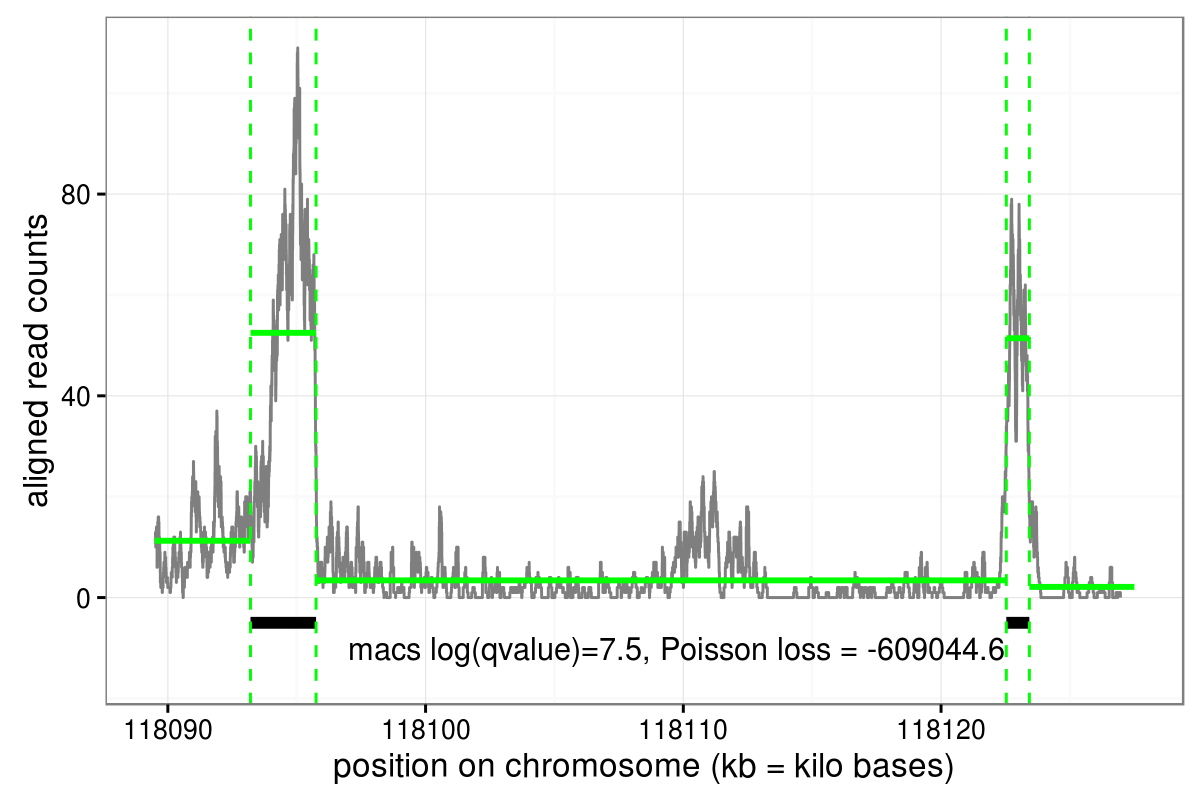
\includegraphics[width=1\textwidth]{figure-macs-problem-7-5.png}
  % $\PoissonLoss(\mathbf z, \mathbf m) = \sum_{i=1}^n m_i - z_i \log(m_i)$
  % for count data $\mathbf z\in\ZZ_+^n$ 
  % and segment mean model $\mathbf m\in\RR^n$.
\end{frame}

\begin{frame}
  \frametitle{Idea: choose the parameter with a lower loss}
  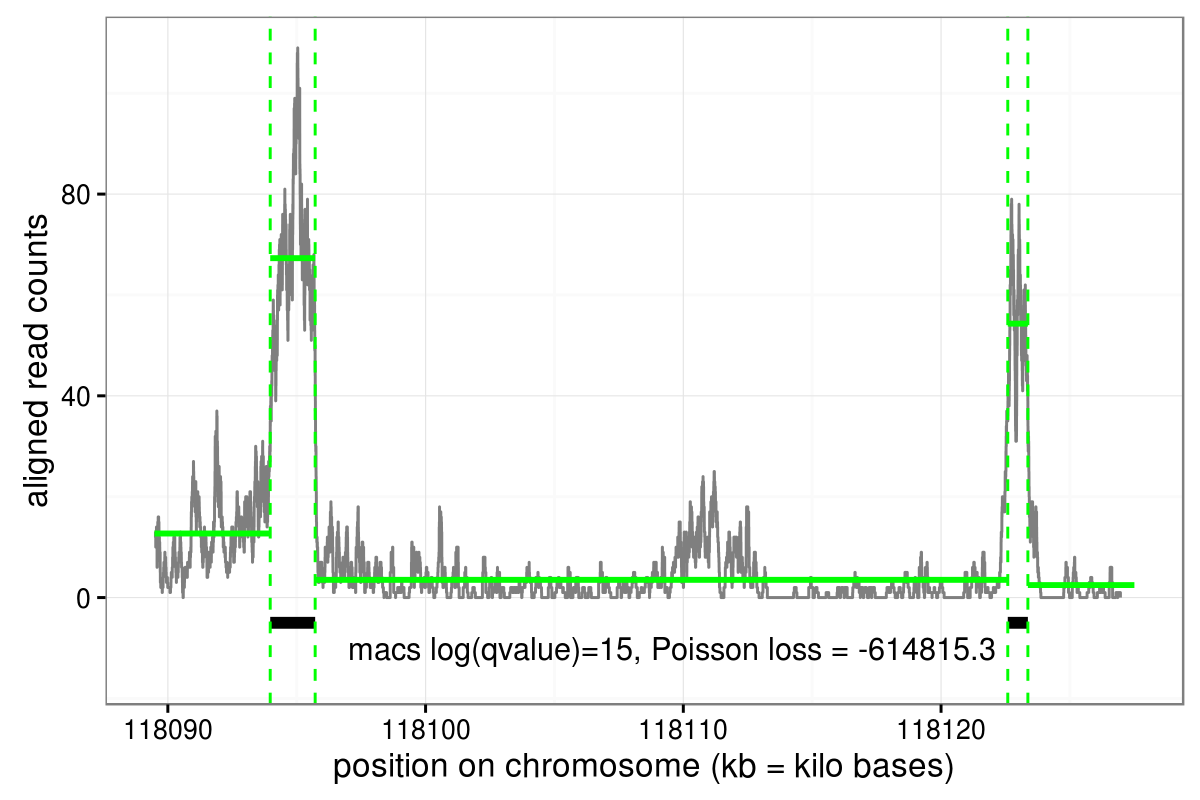
\includegraphics[width=1\textwidth]{figure-macs-problem-15.png}
\end{frame}

\begin{frame}
  \frametitle{PeakSeg: search for the peaks with lowest loss}
  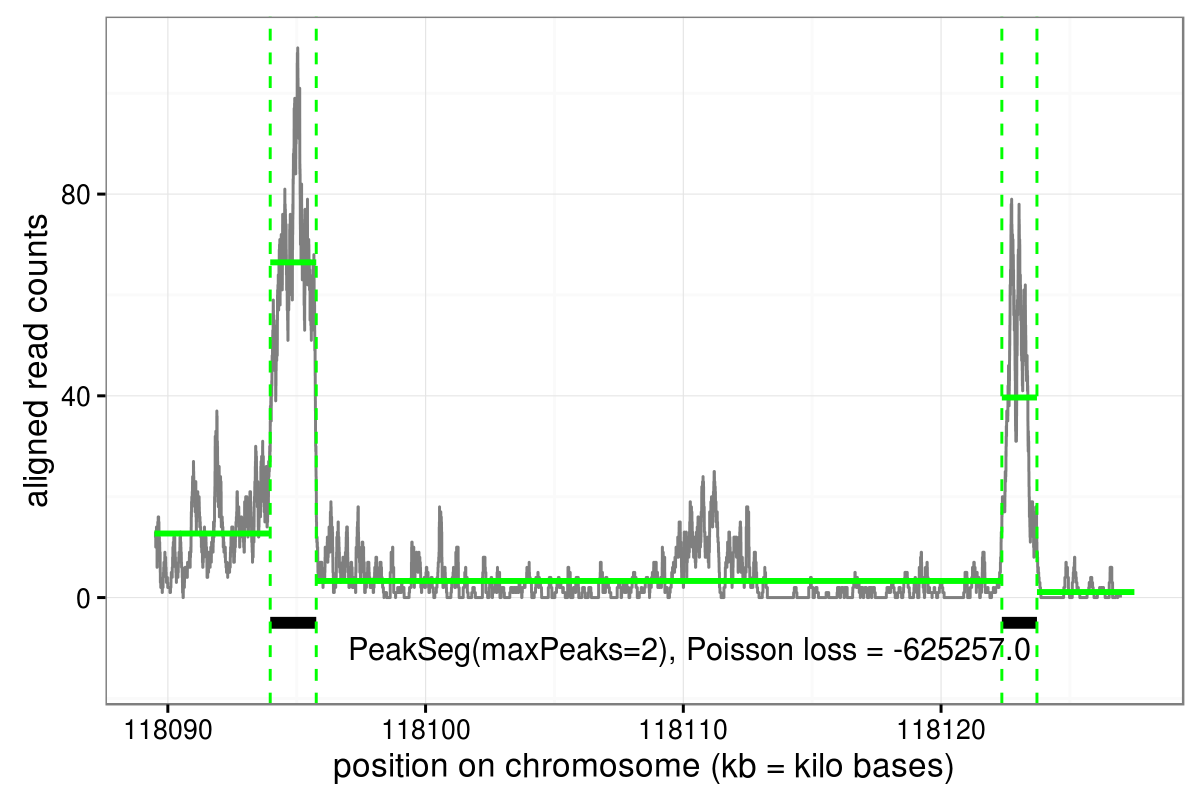
\includegraphics[width=1\textwidth]{figure-macs-problem-PeakSeg.png}

  Simple model with only one parameter (number of peaks).

  %Choose the number of peaks via standard penalties (AIC, BIC,
  %  ...)\\or learned penalties based on visual labels (more on this later).
\end{frame}

% \begin{frame}
%   \frametitle{Maximum likelihood Poisson segmentation models}
%   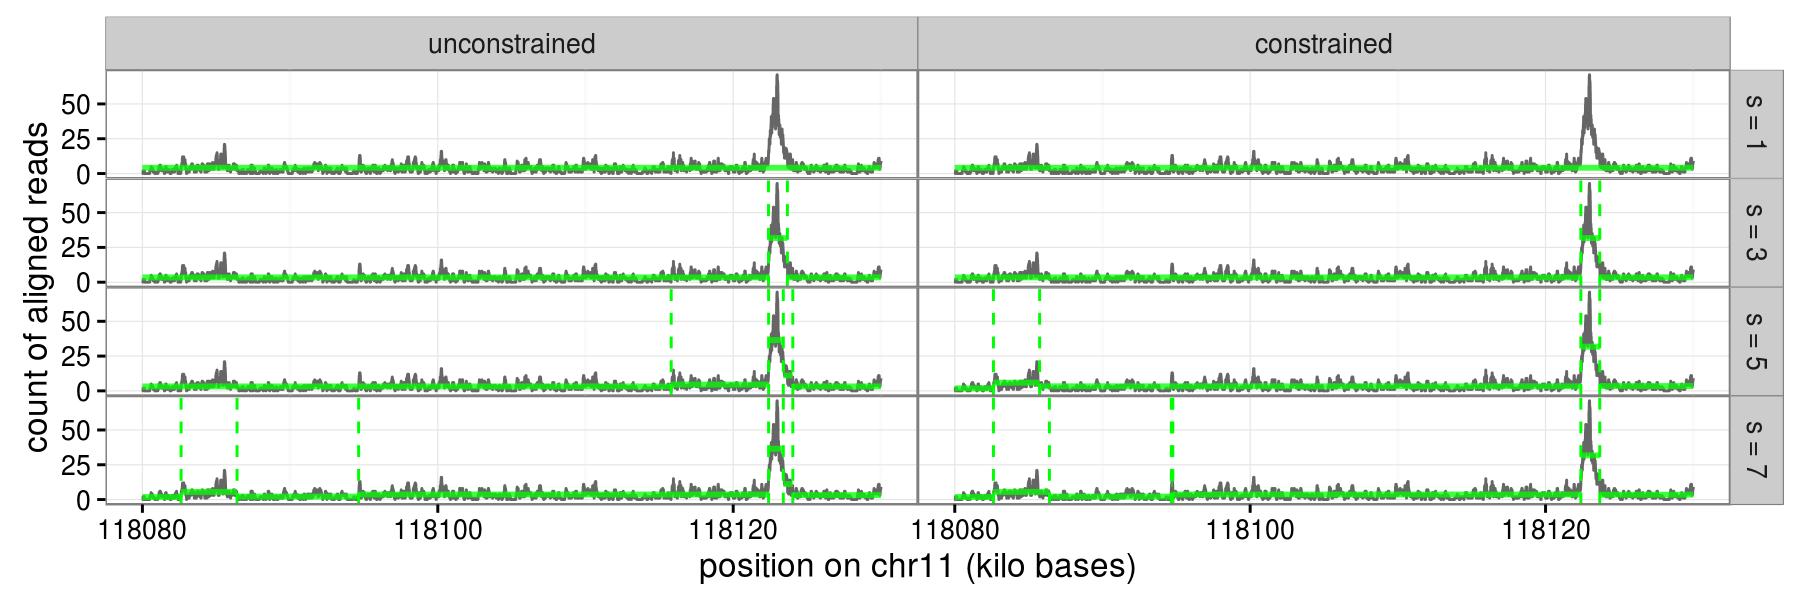
\includegraphics[width=1\textwidth]{figure-Segmentor-PeakSeg}

%   \begin{itemize}
%   \item Previous work: unconstrained maximum likelihood mean\\
%     for $s$ segments ($s-1$ changes), Cleynen et al 2014.
%   \item Hocking et al, ICML 2015: PeakSeg constraint enforces up, down, up,
%     down changes (and not up, up, down). 
%   \item Odd-numbered segments are background noise,\\
%     even-numbered segments are peaks.
%   \item Constrained Dynamic Programming Algorithm, $O(n^2)$ time for $n$ data points.
%   \end{itemize}
% \end{frame}

% \begin{frame}
%   \frametitle{But quadratic time is not fast enough for genomic data!}
%   \includegraphics[width=\textwidth]{figure-PDPA-timings-dp}
%   \begin{itemize}
%   \item Genomic data is large, $n \geq 10^6$.
%   \item Split into subsets? What if we split a peak in half?
%   \item Need linear time algorithm for analyzing whole data set.
%   \end{itemize}
% \end{frame}

\begin{frame}
  \frametitle{Statistical model is a piecewise constant Poisson mean}
  H {\it et al.}, {\it ICML} 2015. 


  \begin{itemize}
  \item We have $n$ count data $z_1, \dots, z_n\in\ZZ_+$.
  \item Fix the number of segments $S\in\{1, 2, \dots, n\}$.
  \item Optimization variables: $S-1$ changepoints
    $t_1 < \cdots < t_{S-1}$ and $S$ segment means $u_1,\dots,u_S\in\RR_+$.
  \item Let $0=t_0<t_1 < \cdots < t_{S-1}<t_S=n$ be the segment
    limits.
  \item Statistical model: for every segment $s\in\{1,\dots,S\}$,
    $z_i \stackrel{\text{iid}}{\sim} \text{Poisson}(u_s)$ for every data
    point $i\in(t_{s-1},t_s]$.
  \item PeakSeg up-down constraint: $u_1\leq u_2 \geq u_3 \leq u_4 \geq \cdots$
  \item Want to find means $u_s$ which maximize the Poisson likelihood:
    $P(Z = z_i|u_s) = u_s^{z_i} e^{-u_s} / (z_i!)$.
  \item Equivalent to finding means $u_s$ which minimize the Poisson
    loss: $\ell(u_s, z_i) = u_s - z_i\log u_s$.
  % \item Comparison to Hidden Markov Model:
  %   \begin{description}
  %   \item[Likelihood] Same emission terms, no transition terms.
  %   \item[Constraint] Number of changes rather than values.
  %   \end{description}
  \end{itemize}
\end{frame}

\begin{frame}
  \frametitle{Dynamic programming and functional pruning}
  \textbf{Classical dynamic programming for optimal partitioning}
  (Jackson et al 2005) computes the vector of optimal loss values up
  to $N$ data points, $O(N^2)$ time because each DP iteration needs to
  consider all $O(N)$ possible changepoints and cost values.
$$
\begin{array}{ccccc}
  \mathcal C_{1} & \mathcal C_2 & \cdots & \mathcal C_{N-1} &  \mathcal C_N
\end{array}
$$
\textbf{Functional pruning optimal partitioning} (Maidstone 2016)
computes a vector of loss \textbf{functions}, $O(N\log N)$ because
each DP iteration only considers $O(\log N)$ candidate changepoints
\\(the others --- which will never be optimal --- are pruned).
$$
\begin{array}{ccccc}
   C_{1}(m_1) & C_2(m_2) & \cdots & C_{N-1}(m_{N-1}) &   C_N(m_{N})
\end{array}
$$
\textbf{Contribution of this work}: a new algorithm that applies the
functional pruning technique to the up-down constrained model.
\end{frame}

\begin{frame}
  \frametitle{Constrained optimal partitioning problem}
  \begin{align*}
  \label{eq:penalized_peakseg}
  \minimize_{
    \substack{
    \mathbf m\in\RR^N,\ \mathbf s\in\{0, 1\}^N\\
\mathbf c\in\{-1, 0,1\}^{N-1}\\
}
    } &\ \ 
  \sum_{i=1}^N \ell(m_i, z_i) + \lambda \sum_{i=1}^{N-1} I(c_i \neq 0) \\
  \text{subject to\ \ } &\ \text{no change: }c_t = 0 \Rightarrow m_t = m_{t+1}\text{ and }s_t=s_{t+1}
  \nonumber\\
&\ \text{go up: }c_t = 1 \Rightarrow m_t \leq m_{t+1}\text{ and }(s_t,s_{t+1})=(0,1),
  \nonumber\\
&\ \text{go down: } c_t = -1 \Rightarrow m_t \geq m_{t+1}\text{ and }(s_t,s_{t+1})=(1,0).
\nonumber
\end{align*}
\begin{minipage}{0.5\linewidth}
    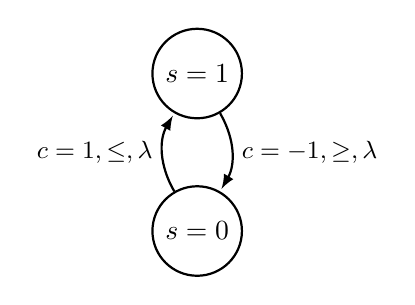
\begin{tikzpicture}[->,>=latex,shorten >=1pt,auto,node distance=2cm,
                    thick,main node/.style={circle,draw}]

  \node[main node] (1) {$s=1$};
  \node[main node] (2) [below of=1] {$s=0$};

  \path[every node/.style={font=\sffamily\small}]
    (2) edge [bend left] node {$c=1, \leq, \lambda$} (1)
    (1) edge [bend left] node {$c=-1, \geq, \lambda$} (2);
\end{tikzpicture}
\end{minipage}
\begin{minipage}{0.45\linewidth}
  Nodes=states $s$,\\
  Edges=changes $c$ (constraint, penalty).
\end{minipage}
\end{frame}

\begin{frame}
  \frametitle{Generalized Functional Pruning Optimal Partitioning
    (GFPOP) algorithm for up-down constrained model}
Recursively compute two vectors of real-valued cost functions:
$$
\begin{array}{cccl}
  \overline C_{1}(m_1) & \cdots & \overline C_N(m_{N})& \text{ optimal cost in peak state $s=1$}\\
  \underline C_{1}(m_1) & \cdots & \underline C_N(m_{N})& \text{ optimal cost in background state $s=0$}\\
\end{array}
$$
\begin{minipage}{0.65\linewidth}
  $$\overline C_{t+1}(\mu) = \ell(\mu, z_i) + \min\{
  \overline C_t(\mu),\, 
  \underline C_t^\leq(\mu)+\lambda
\},$$
  $$\underline C_{t+1}(\mu) = \ell(\mu, z_i) + \min\{
  \underline C_t(\mu),\, 
  \overline C_t^\geq(\mu)+\lambda
\},$$
where $f^\leq(\mu) = \min_{x\leq\mu} f(x)$,\\
$f^\geq(\mu) = \min_{x\geq\mu} f(x)$.
\end{minipage}
\begin{minipage}{0.25\linewidth}
  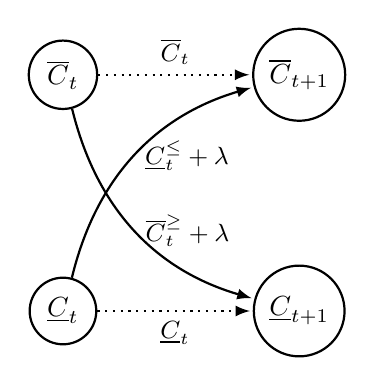
\begin{tikzpicture}[->,>=latex,shorten >=1pt,auto,node distance=3cm,
  thick,main node/.style={circle,draw}]
  \node[main node] (peak_t) {$\overline C_t$};
  \node[main node] (bkg_t) [below of=peak_t] {$\underline C_t$};
  \node[main node] (peak_t1) [right of=peak_t] {$\overline C_{t+1}$};
  \node[main node] (bkg_t1) [right of=bkg_t] {$\underline C_{t+1}$};
  \path[every node/.style={font=\small}]
    (peak_t) edge [dotted] node {$\overline C_{t}$} (peak_t1)
    (peak_t) edge [black, bend right] node [right] {$\overline C_{t}^{\geq}+\lambda$} (bkg_t1)
    (bkg_t) edge [dotted] node[midway, below] {$\underline C_{t}$} (bkg_t1)
    (bkg_t) edge [black, bend left] node[right] {$\underline C_{ t}^{\leq}+\lambda$} (peak_t1)
;
\end{tikzpicture}
\end{minipage}
\end{frame}




\end{document}
